%%%%%%%%%%%%%%%%%%%%%%%%%%%%%%%%%%%%%%%%%
% TMESC Dissertation
% LaTeX Template
% Version 0.2 (Aug/2023)
%
% Adapted to MESCC/ISEP (Apr/2023, Aug/2023 & Nov/2023) by
% Luis Miguel Pinho
%
% Based on TMDEI/ISEP style (Dec/2015) by
%  Nuno Pereira (nap@isep.ipp.pt) and
%  Paulo Baltarejo (pbs@isep.ipp.pt)
%
% Based on MastersDoctoralThesis Version 1.2 by Vel (vel@latextemplates.com) and
% Johannes Böttcher, downloaded from (21/11/15):
% http://www.LaTeXTemplates.com
%
% This template is originally based on a template by:
% Steve Gunn (http://users.ecs.soton.ac.uk/srg/softwaretools/document/templates/)
% Sunil Patel (http://www.sunilpatel.co.uk/thesis-template/)
%
% Template license:
% CC BY-NC-SA 3.0 (http://creativecommons.org/licenses/by-nc-sa/3.0/)
%
%%%%%%%%%%%%%%%%%%%%%%%%%%%%%%%%%%%%%%%%%

%----------------------------------------------------------------------------------------
%	PACKAGES AND OTHER DOCUMENT CONFIGURATIONS
%----------------------------------------------------------------------------------------

\documentclass[
11pt, % The default document font size, options: 10pt, 11pt, 12pt
%oneside, % Two side (alternating margins) for binding by default, uncomment to switch to one side (for drafting/reading purposes)
english, % english for English;
%portuguese,% for Portuguese; delete temporary files if you change language (e.g. 'make clean; make')
singlespacing, % Single line spacing, alternatives: onehalfspacing or doublespacing (for drafting/reading purposes)
%draft, % Uncomment to enable draft mode (no pictures, no links, overfull hboxes indicated)
%nolistspacing, % If the document is onehalfspacing or doublespacing, uncomment this to set spacing in lists to single
liststotoc, % Uncomment to add the list of figures/tables/etc to the table of contents (not recommended)
%toctotoc, % Uncomment to add the main table of contents to the table of contents (not recommended)
parskip, % Add space between paragraphs (recommended)
%nohyperref, % Uncomment to not load the hyperref package (not recommended)
nohyperreflinkcolor, % hyperref links are not colored (comment to color links, for example to produce an electronic-only version)
headsepline, % Uncomment to get a line under the header
]{tmesc-style} % The class file specifying the document structure

\usepackage{tikz} % Required for creating graphics programmatically (can be removed if not used)
%\usetikzlibrary{arrows} % Required for fancy arrows in TiKZ graphics (can be removed if not used)

\usepackage{pgfplots} % Required for drawing high--quality function plots (can be removed if not used)
\pgfplotsset{compat=newest}
%
% Next you have examples of admissable citation styles; we recomend using the authoryear-comp citation style (which resembles Harvard); don't forget to only uncomment one
%

% authoryear-comp: recommended citation style (e.g. (Buendía, 1860), (Buendía 1910, Arcadio 1940))
\usepackage[style=authoryear-comp,backend=biber]{biblatex} % Bibtex backend with the authoryear-comp citation style (authoryear citations, bibliography ordered alphabetically)

% numeric citation style (e.g. [1], [1-3])
%\usepackage[style=numeric-comp,sorting=none,backend=biber]{biblatex} % Bibtex backend with the numeric-comp citation style (numeric citations, bibliography ordered by appearance)

% alphabetic citation style (e.g. [Buendía10], [Buendía10, Arcadio40])
%\usepackage[style=alphabetic,sorting=none,backend=biber]{biblatex} % Bibtex backend with the alphabetic citation style (alphabetic citations, bibliography ordered by appearance)
\usepackage{scrhack} 
\usepackage{placeins}
\usepackage{booktabs}
\usepackage{parskip}
\usepackage{mathptmx}
\usepackage{helvet}
\usepackage{lmodern}
% Listings for code highlighting
\usepackage{listings}
\usepackage{xcolor}
% Import the comment package
\usepackage{comment} 
%To put my debug
\usepackage{verbatim}



% Define Rust language settings for listings
\lstdefinelanguage{Rust}{
  keywords={fn, let, mut, impl, struct, enum, use, pub, crate, match, if, else, while, for, loop, break, continue, return},
  keywordstyle=\color{blue},
  stringstyle=\color{red},
  commentstyle=\color{green},
  morecomment=[l][\color{magenta}]{//},
  morecomment=[s][\color{magenta}]{/*}{*/},
  morestring=[b]',
  morestring=[b]",
}

\lstset{
  language=Rust,
  basicstyle=\ttfamily\footnotesize,
  numbers=left,
  numberstyle=\tiny,
  stepnumber=1,
  numbersep=5pt,
  backgroundcolor=\color{gray!10},
  frame=single,
  captionpos=b,
  breaklines=true
}




%%% AMB: ADICIONEI O PACOTE TODONOTES PARA ADICIONAR COMENTÁRIOS DE FORMA VISÍVEL, FÁCEIS DE APAGAR NA VERSÃO FINAL
% USAR A LINHA SEGUINTE PARA MOSTRAR OS COMENTÁRIOS, CASO CONTRÁRIO COMENTAR.
%\usepackage{todonotes}
% USAR A LINHA SEGUINTE PARA OCULTAR OS COMENTÁRIOS, CASO CONTRÁRIO COMENTAR.
\usepackage[disable]{todonotes}

\addbibresource{mainbibliography.bib} % The filename of the bibliography
%\usepackage[acronym]{glossaries}
\makeglossaries % build the glossary

%----------------------------------------------------------------------------------------
%	THESIS INFORMATION
%----------------------------------------------------------------------------------------

\thesistitle{Real-Time Quality Index Estimation for Redundant Sampled Values Streams in Digital Substations} % Your thesis title, this is used in the title, print it elsewhere with \ttitle

%\thesissubtitle{{[}Subtitle (if exists){]}} % Your thesis subtitle, this is used in the title, print it elsewhere with \tsubtitle, comment line if not existing

\author{Everton Matheus Oriente} % Your name, this is used in the title page, print it elsewhere with \authorname

\supervisor{António Manuel de Sousa Barros} % Your supervisor's name, this is used in the title page, print it elsewhere with \supname

\committeepresident{Luís Miguel Pinho, Professor Coordenador, Instituto Superior de Engenharia do Porto} % Name of the president of the evaluation committee, print it elsewhere with \presidentname

\committeemembers{Ricardo Severino, Professor Adjunto, Instituto Superior de Engenharia do Porto \\ António Barros, Professor Adjunto, Instituto Superior de Engenharia do Porto} % Name of the evaluation committee members (up to four), print it elsewhere with \committee

\keywords{IEC61850-9-2 Sampled Values, Intelligent Electronic Devices (IED) and Protection Relays} % Please define up to 6 keywords that better describe your work, print it elsewhere with \keywordnames

\thesisdate{Porto, \today} % thesis date,  print it elsewhere with \tdate

\hypersetup{pdftitle=\ttitle} % Set the PDF's title to your title
\hypersetup{pdfauthor=\authorname} % Set the PDF's author to your name
\hypersetup{pdfkeywords=\keywordnames} % Set the PDF's keywords to your keywords

\begin{document}

\nocite{*}

%----------------------------------------------------------------------------------------
%	FRONT MATTER
%----------------------------------------------------------------------------------------

% Include the frontmatter of your thesis here

% we include the glossary here (frontmatter is included with \input, so this command is as if it was in main.tex)
%All acronyms must be written in this file.
\newacronym{acsi}{ACSI}{Abstract Communication Service Interface}
\newacronym{ascii}{ASCII}{American Standard Code for Information Interchange}
\newacronym{cb}{CB}{Circuit Breaker}
\newacronym{ct}{CT}{Current Transformer} 
\newacronym{goose}{GOOSE}{Generic Object Oriented Substation Events}
\newacronym{iec}{IEC}{International Electrotechnical Commission}
\newacronym{ied}{IED}{Intelligent Electronic Devices}
\newacronym{ieee}{IEEE}{Institute of Electrical and Electronic Engineers}
\newacronym{irigb}{IRIG-B}{Inter-Range Instrumentation Group}
\newacronym{ip}{IP}{Internet Protocol}
\newacronym{lan}{LAN}{Local Area Network}
\newacronym{ld}{LD}{Logical Device}
\newacronym{ln}{LN}{Logical Node}
\newacronym{mms}{MMS}{Manufacturing Message Specification}
\newacronym{os}{OS}{Operating System}
\newacronym{ptp}{PTP}{Precision Time Protocol}
\newacronym{rtos}{RTOS}{Real-Time Operating System}
\newacronym{sas}{SAS}{Substation Automation Systems}
\newacronym{scada}{SCADA}{Supervisory Control and Data Acquisition}
\newacronym{scl}{SCL}{Substation Configuration description Language}
\newacronym{scsm}{SCSM}{Specific Communication Service Mapping}
\newacronym{sw}{SW}{Disconnector}
\newacronym{sv}{SV}{Sampled-Values}
\newacronym{tcp}{TCP}{Transmission Control Protocol}
\newacronym{udp}{UDP}{User Datagram Protocol}
\newacronym{vt}{VT}{Voltage Transformer}



\frontmatter % Use roman page numbering style (i, ii, iii, iv...) for the pre-content pages

\pagestyle{plain} % Default to the plain heading style until the thesis style is called for the body content

%----------------------------------------------------------------------------------------
%	TITLE PAGE
%----------------------------------------------------------------------------------------
%\sloppy
\maketitlepage


%----------------------------------------------------------------------------------------
%	STATEMENT of INTEGRITY
%----------------------------------------------------------------------------------------
\integritystatement

%----------------------------------------------------------------------------------------
%	DEDICATION  (optional)
%----------------------------------------------------------------------------------------
%
%\dedicatory{For/Dedicated to/To my\ldots}
%\begin{dedicatory}
%The dedicatory is optional. 
%\end{dedicatory}

%----------------------------------------------------------------------------------------
%	ABSTRACT PAGE
%----------------------------------------------------------------------------------------

\begin{abstract}
	
	%\sloppy
	%\raggedright
	% here you put the abstract in the main language of the work.
	
	%With the advancement of technology, electromechanical relays have evolved into Intelligent Electronic Devices (IEDs) and, as a result, protection relays have gained the ability to communicate. They not only provide equipment protection but also communicate with other devices and exchange information among themselves.
	Protection devices are essential elements in the electric power grid, as they safeguard equipment and ensure the stability and reliability of the network by detecting faults and preventing damage through timely isolation of affected areas.
	With technological advancements, electromechanical protection relays have evolved into Intelligent Electronic Devices (IEDs), essentially protection relays with built-in communication capabilities.
	These modern relays not only protect equipment but also exchange critical information with other devices.
	
	%Communication protocols bring many advantages and challenges.
	%They reduce the amount of wiring needed to transmit information.
	%Previously, a wire was required for each piece of information, but with communication protocols, a pair of wires is sufficient to convey various pieces of information. However, the knowledge required to implement this is significantly greater.
	However, the variety of events and data exchanged between power grid components is substantial.
	In this respect, communication protocols present both advantages and challenges.
	On one hand, they enable the signalling of diverse events and the transmission of multiple pieces of information over a single medium.
	On the other hand, a protocol is only effective if all components within the system comply with it.
	
	%With the introduction of the IEC61850 protocol, the energy sector has established a communication standard for the entire segment. This protocol has brought interoperability among manufacturers, one of the numerous advantages it has over other protocols. Real-time information exchange occurs through specific protocols that are part of the IEC 61850 standard, ensuring higher data quality and availability.
	The introduction of the IEC~61850 protocol has established a unified communication standard across the energy sector.
	This protocol promotes interoperability between manufacturers, offering significant advantages over other standards.
	Real-time data exchange is facilitated by specific protocols within the IEC 61850 framework, which specifically address the communication requirements of IEDs, ensuring enhanced data quality and availability.
	%Now, a customer is no longer bound to a single manufacturer, not having to replace all equipment when upgrading devices. This is because all devices are required to communicate following the established protocol. As Intelligent Electronic Devices play a critical role in substations, and many of their functions are critical and need to be executed at the right time, any development incorporated into the device has an impact on the entire product.
	
	As IEDs play a crucial role in substations, with many of their functions being both critical and time-sensitive, any developments incorporated into these devices can significantly impact the entire system.
	An IED analyses the stream of Sampled Values (SVs) sent by a Merging Unit to detect faults and implement protective measures.
	The Merging Unit sends SVs over two independent channels: the primary and the secondary (redundant) channels.
	When the primary channel fails, the secondary channel takes over, ensuring the information that the primary channel could not transmit is conveyed.
	As such, the current decision-making process for switching channels is based solely on the occurrence of a total channel failure.
	
	This thesis aims to enhance IED functionality by adding intelligence to this channel selection method.
	It proposes ways to evaluate, quantify, and qualify the received information to determine the most reliable signal source, whether from Channel 1 (primary) or Channel 2 (secondary).
	This approach ensures that protection relays receive better information, enabling protection algorithms to act correctly and promptly within their operating parameters.
	
	\todo[inline]{AMB: Modifiquei o ABSTRACT de forma a remover texto redundante, e ligando algumas ideias de forma mais fluída.}
	\todo[inline]{AMB: Nas keywords "Sampled Values" não me parece uma boa palavra-chave. "Intelligent Electronic Devices" e "Protection Relays" (ou um termo mais técnico são boas palavras-chave.}
	\todo[inline]{AMB: Aprovando esta versão do Abstract, é ir ao Google Translate ou ao ChatGPT e pedir para traduzir o texto para português.}
	
	%This thesis aims to develop a new functionality for IEDs.
	%Currently, the treatment for SV's (Sampled Values) in the protection relay involves checking communication with the Merging Unit, which acquires and sends information to the protection relays.
	%When the primary channel fails to transmit, the secondary channel takes over, informing the protection relay about the information that the first channel failed to send.
	%If one channel fails, the other can provide the lost information and assume the primary communication.
	
	%For example, the channel 1 provides information as the primary channel.
	%As soon as Channel 1 is interrupted for any reason, Channel 2 takes over, providing information to the protection relay.
	%This is the decision-making method; when there is a total system failure, the other channel assumes control.
	%The proposed functionality in this master's thesis aims to add intelligence to this selection method by suggesting ways to evaluate, quantify, and qualify the received information.
	%It aims to determine which signal to use based on indicators, whether through Channel 1 (primary) or Channel 2 (secondary).
	%This ensures better information for protection relays, allowing protection algorithms to take the correct actions as quickly as possible within their operating parameters.
	
	%It is through Sample Values that protection algorithms determine if there is a fault in the electrical network, becoming a highly critical component for the entire system with a direct impact on product performance in terms of quality, efficiency, and reliability.
	%%%%%%%%%%
	
	%As IEDs play a crucial role in substations, with many of their functions being both critical and time-sensitive, any developments incorporated into these devices can have a significant impact on the entire system.
	%This thesis aims to develop a new functionality for IEDs.
	%Currently, the treatment for SV's (Sampled Values) in the protection relay involves checking communication with the Merging Unit, which acquires and sends information to the protection relays.
	%When the primary channel fails to transmit, the secondary channel takes over, informing the protection relay about the information that the first channel failed to send.
	%If one channel fails, the other can provide the lost information and assume the primary communication.
	
	%For example, the channel 1 provides information as the primary channel.
	%As soon as Channel 1 is interrupted for any reason, Channel 2 takes over, providing information to the protection relay.
	%This is the decision-making method; when there is a total system failure, the other channel assumes control.
	%The proposed functionality in this master's thesis aims to add intelligence to this selection method by suggesting ways to evaluate, quantify, and qualify the received information.
	%It aims to determine which signal to use based on indicators, whether through Channel 1 (primary) or Channel 2 (secondary).
	%This ensures better information for protection relays, allowing protection algorithms to take the correct actions as quickly as possible within their operating parameters.
	
	%It is through Sample Values that protection algorithms determine if there is a fault in the electrical network, becoming a highly critical component for the entire system with a direct impact on product performance in terms of quality, efficiency, and reliability.
	
\end{abstract}

\begin{abstractotherlanguage}
	% here you put the abstract in the "other language": English, if the work is written in Portuguese; Portuguese, if the work is written in English.
	
	Relés de proteção são elementos essenciais na rede elétrica, pois protegem os equipamentos e garantem a estabilidade e confiabilidade da rede, detectando falhas e prevenindo danos através da isolação oportuna das áreas afetadas.
	
	Com os avanços tecnológicos, os relés de proteção eletromecânicos evoluíram para Dispositivos Eletrônicos Inteligentes (IEDs), essencialmente relés de proteção com capacidades de comunicação integradas. Esses relés modernos não apenas protegem os equipamentos, mas também trocam informações críticas com outros dispositivos.
	
	No entanto, a variedade de eventos e dados trocados entre os componentes da rede elétrica é substancial. Nesse aspecto, os protocolos de comunicação apresentam tanto vantagens quanto desafios. Por um lado, eles permitem a sinalização de diversos eventos e a transmissão de múltiplas informações através de um único meio. Por outro lado, um protocolo só é eficaz se todos os componentes do sistema o seguirem.
	
	A introdução do protocolo IEC 61850 estabeleceu um padrão de comunicação unificado no setor energético. Esse protocolo promove a interoperabilidade entre fabricantes, oferecendo vantagens significativas sobre outros padrões. A troca de dados em tempo real é facilitada por protocolos específicos dentro da estrutura do IEC 61850, que atendem às exigências de comunicação dos IEDs, garantindo uma melhor qualidade e disponibilidade dos dados.
	
	Como os IEDs desempenham um papel crucial nas subestações, com muitas de suas funções sendo críticas e sensíveis ao tempo, qualquer desenvolvimento incorporado a esses dispositivos pode impactar significativamente todo o sistema. Um IED analisa o fluxo de Valores Amostrados (SVs) enviados por uma Unidade de Mesclagem para detectar falhas e implementar medidas de proteção. A Unidade de Mesclagem envia SVs por dois canais independentes: o canal primário e o canal secundário (redundante). Quando o canal primário falha, o canal secundário assume, garantindo que a informação que o canal primário não pôde transmitir seja transmitida.
	
	Assim, o processo de tomada de decisão atual para a troca de canais baseia-se unicamente na ocorrência de uma falha total do canal.
	
	Esta tese tem como objetivo aprimorar a funcionalidade dos IEDs, adicionando inteligência a esse método de seleção de canal. Propõe maneiras de avaliar, quantificar e qualificar a informação recebida para determinar a fonte de sinal mais confiável, seja do Canal 1 (primário) ou do Canal 2 (secundário). Essa abordagem garante que os relés de proteção recebam informações de melhor qualidade, permitindo que os algoritmos de proteção atuem de forma correta e rápida dentro dos seus parâmetros de operação.
		
\end{abstractotherlanguage}

%----------------------------------------------------------------------------------------
%	ACKNOWLEDGEMENTS (optional)
%----------------------------------------------------------------------------------------

\begin{acknowledgements}
	
I would like to express my deepest gratitude to my wife, Graziela Preisegalavicius, for her unwavering support and encouragement throughout this journey. Your patience, love, and understanding have been my greatest source of strength.

To my son, Theo Preisegalavicius Oriente, thank you for bringing endless joy into my life and giving me the motivation to push forward. Your smiles and laughter have been my driving force.

I am also profoundly grateful to my parents, Irani Matheus Oriente and Hamilton Angelo Oriente, for their lifelong support and guidance. Your belief in me has been the foundation upon which I have built my achievements.

Finally, I would like to extend my sincere thanks to my supervisor, Antonio Barros, for his insightful guidance and encouragement throughout the development of this thesis.
	
\end{acknowledgements}

%----------------------------------------------------------------------------------------
%	LIST OF CONTENTS/FIGURES/TABLES PAGES
%----------------------------------------------------------------------------------------

\tableofcontents % Prints the main table of contents

\listoffigures % Prints the list of figures

%\listoftables % Prints the list of tables

%\iflanguage{portuguese}{
%	\renewcommand{\listalgorithmname}{Lista de Algor\'itmos}
%}
%\listofalgorithms % Prints the list of algorithms
%\addchaptertocentry{\listalgorithmname}


\renewcommand{\lstlistlistingname}{List of Source Code}
\iflanguage{portuguese}{
	\renewcommand{\lstlistlistingname}{Lista de C\'odigo}
}
\lstlistoflistings % Prints the list of listings (programming language source code)
\addchaptertocentry{\lstlistlistingname}


%----------------------------------------------------------------------------------------
%	ABBREVIATIONS
%----------------------------------------------------------------------------------------
\begin{abbreviations}{ll} % Include a list of abbreviations (a table of two columns)
\textbf{ACSI} & \textbf{A}bstract \textbf{C}ommunication \textbf{S}ervice \textbf{I}nterface \\
\textbf{ASCII} & \textbf{A}merican \textbf{S}tandard \textbf{C}ode for \textbf{I}nformation \textbf{I}nterchange \\
\textbf{CB} & \textbf{C}ircuit \textbf{B}reaker \\
\textbf{CT} & \textbf{C}urrent \textbf{T}ransformer \\
\textbf{GOOSE} & \textbf{G}eneric \textbf{O}bject \textbf{O}riented \textbf{S}ubstation \textbf{E}vents \\
\textbf{IEC} & \textbf{I}nternational \textbf{E}lectrotechnical \textbf{C}ommission \\
\textbf{IED} & \textbf{I}ntelligent \textbf{E}lectronic \textbf{D}evices \\
\textbf{IEEE} & \textbf{I}nstitute of \textbf{E}lectrical and \textbf{E}lectronic \textbf{E}ngineers \\
\textbf{IRIG-B} & \textbf{I}nter-\textbf{R}ange \textbf{I}nstrumentation \textbf{G}roup \\
\textbf{IP} & \textbf{I}nternet \textbf{P}rotocol \\
\textbf{LAN} & \textbf{L}ocal \textbf{A}rea \textbf{N}etwork \\
\textbf{LD} & \textbf{L}ogical \textbf{D}evice \\
\textbf{LN} & \textbf{L}ogical \textbf{N}ode \\
\textbf{MMS} & \textbf{M}anufacturing \textbf{M}essage \textbf{S}pecification \\
\textbf{OS} & \textbf{O}perating \textbf{S}ystem \\
\textbf{PTP} & \textbf{P}recision \textbf{T}ime \textbf{P}rotocol \\
\textbf{RTOS} & \textbf{R}eal-\textbf{T}ime \textbf{O}perating \textbf{S}ystem \\
\textbf{SAS} & \textbf{S}ubstation \textbf{A}utomation \textbf{S}ystems \\
\textbf{SCADA} & \textbf{S}upervisory \textbf{C}ontrol and \textbf{D}ata \textbf{A}cquisition \\
\textbf{SCL} & \textbf{S}ubstation \textbf{C}onfiguration description \textbf{L}anguage \\
\textbf{SCSM} & \textbf{S}pecific \textbf{C}ommunication \textbf{S}ervice \textbf{M}apping \\
\textbf{SW} & \textbf{D}isconnector \\
\textbf{SV} & \textbf{S}ampled-\textbf{V}alues \\
\textbf{TCP} & \textbf{T}ransmission \textbf{C}ontrol \textbf{P}rotocol \\
\textbf{UDP} & \textbf{U}ser \textbf{D}atagram \textbf{P}rotocol \\
\textbf{VT} & \textbf{V}oltage \textbf{T}ransformer \\
\end{abbreviations}

%----------------------------------------------------------------------------------------
%	SYMBOLS
%----------------------------------------------------------------------------------------

%\begin{symbols}{lll} % Include a list of Symbols (a three column table)
	
	% [Note: Although acronyms and symbols are defined in this section, they should also be defined at least the first time used in the dissertation body.]
	
%	$a$ & distance & \si{\meter} \\
%	$P$ & power & \si{\watt} (\si{\joule\per\second}) \\
	%Symbol & Name & Unit \\
	
%	\addlinespace % Gap to separate the Roman symbols from the Greek
	
%	$\omega$ & angular frequency & \si{\radian} \\
	
%\end{symbols}



%----------------------------------------------------------------------------------------
%	ACRONYMS
%----------------------------------------------------------------------------------------

\newcommand{\listacronymname}{List of Acronyms}
\iflanguage{portuguese}{
	\renewcommand{\listacronymname}{Lista de Acr\'onimos}
}

%Use GLS
\glsresetall
\printglossary[title=\listacronymname,type=\acronymtype,style=long]

%----------------------------------------------------------------------------------------
%	DONE
%----------------------------------------------------------------------------------------

\mainmatter % Begin numeric (1,2,3...) page numbering
\pagestyle{thesis} % Return the page headers back to the "thesis" style


%----------------------------------------------------------------------------------------
%	MAIN BODY
%----------------------------------------------------------------------------------------

% Include the chapters of the thesis as separate folder for each chapter
% Uncomment the lines as you write the chapters

% Chapter 1
% 
\chapter{Introduction} % Main chapter title
\label{chap:Chapter1} % For referencing the chapter elsewhere, use Chapter~\ref{Chapter1}


%-------------------------------------------------------------------------------
%---------
%
\section{Overview}
\label{sec:chap1_guidelines} %For referencing this section elsewhere, use Section~\ref{sec:chap1_guidelines}
Since the discovery of electricity, humanity has harnessed electrical energy for a multitude of purposes. As the demand for electricity grew, encompassing applications like heating, ventilation, and lighting, the need to generate more electrical power became paramount to accommodate the evolving array of functionalities that emerged over time.

Consequently, diverse power plants were established to meet the increasing demand. These included thermal power plants, hydroelectric plants, nuclear facilities, geothermal installations, combined-cycle plants, and others. In contemporary times, we have witnessed the advent of novel energy sources, such as wind, solar, tidal, biomass, and green hydrogen. Classified as renewable energies, these sources, along with hydroelectric power, offer a pathway towards planetary decarbonization, as they eschew reliance on fossil fuels.

However, these power-generating facilities often found themselves situated at a considerable distance from major consumers, specifically large urban centers. This spatial disparity necessitated the development of a means to efficiently transport the energy generated by these plants to the significant consumer hubs. This necessity gave rise to electrical substations, pivotal in facilitating the transmission of energy from power plants to end consumers, thereby playing a fundamental role in the entire energy cycle.

However, the introduction of electrical substations takes place, and while various types exist,here spotlight four specific substation categories here:

\begin{itemize}
	\item Step-up substations: Positioned in close proximity to power plants, these substations serve the crucial function of elevating the energy voltage. This strategic placement aims to minimize losses attributable to phenomena such as Foucault currents and parasitic currents, ensuring the delivery of generated power with utmost efficiency. Given the substantial distances involved in transmission, the decision to increase voltage at this stage becomes imperative to effectively mitigate the mentioned challenges.
	
	\item Distribution Substation: Following the transmission of energy from remote areas at higher voltages to minimize losses, it becomes essential to lower the voltage before reaching consumers at safer levels. This leads to distribution substations, where the voltage is reduced, allowing for a more seamless distribution of energy within urban centers.
	
	\item Step-Down Substation: The step-down substation is the one located very close to the end consumer, operating at a lower voltage than in distribution, thereby reducing the risks to the individuals who utilize it.
	
	\item Switching Substation: This facility is designed to interconnect supply circuits operating at the same voltage level. It allows for the segmentation of circuits, facilitating the power on of shorter sections, and enabling a more flexible and efficient distribution of electrical power.
	
\end{itemize}

Figure~\ref{fig:electricity-pathway} is a diagram illustrating the path from the power plant where the energy is generated, going through high power transformer to elevate the voltage to have minimum losses, the transmission line to transmit all the power, a high power transformer to step down the voltage and send the energy to the end consumer,~\footnote{\url{https://www.eia.gov/energyexplained/electricity/delivery-to-consumers.php}}.

\begin{figure}[tbh]
	\centering
	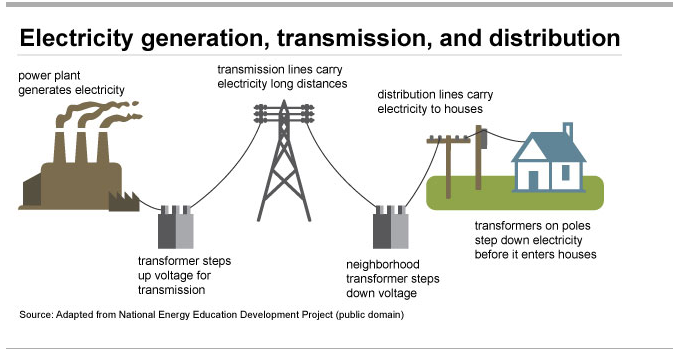
\includegraphics[width=\textwidth, keepaspectratio]{ch1/assets/Way_of_electricity.png}
	\caption{Electricity Generation, Transmission, and Distribution Pathway (Image credits: U.S. Energy Information Administration)}
	\label{fig:electricity-pathway}
\end{figure}

\section{Digital Substation}
Electric power substations play a fundamental role in the entire cycle of electric energy and its transformations. Simultaneously, as we witness several generating sources converting energy, such as hydroelectric (water turbines), thermal (steam turbines), combined cycle (gas turbines and steam turbines), wind (wind energy), solar farms (solar energy), among others into electric energy, numerous consumers draw upon this produced energy. The absence of an energy storage location underscores the substantial importance of substations. Without them, meeting the extensive demand and need for electric energy would be impracticable, hindering economic growth and the development of industries, businesses, and even entire countries. Today, every facet of operation, from mega-factories to simple light bulbs, relies on electric energy.

Substations facilitate the extended reach of energy to diverse locations, enabling a direct connection from the generating source to consumers. Serving as the link between generation and consumption, substations categorize the electric energy chain into four major divisions: electric energy generation, electric energy transmission, electric energy distribution, and electric energy consumption. These processes start with High Voltage (Generation), increases to Very High Voltage (Transmission), goes to Medium Voltage (Distribution) and when finally reaches the consumer is Low Voltage (Consumers).

The evolution of electric substations has embraced new technologies, as preventive maintenance, predictability of problem occurrences, fault alerts, backyard equipment switching, and visualization of currents and voltages. Follow these advancements are electromechanical protection relays, monitoring and safeguarding against electrical faults in backyard equipment.
Backyard equipment, including high-voltage circuit breakers, switches, capacitor banks, reactors, transformers, and transmission lines, retains the basic concept from the 1990s but now has features enhanced performance and added functionalities due to technological advances.

Electric power systems within a substation can be categorized into four levels:

\begin{itemize}
	\item Level 0 - Backyard Equipment: Encompassing all devices responsible for transmitting energy from the power generation station to customers, factories, public lighting, residences, hospitals, data centers, etc. These devices are responsible for the entire energy system.
	\item Level 1 - Protection Relays: Formerly known as Intelligent Electronic Devices (IED), these devices have replaced the need for multiple protection relays, executing a lot of protection functions, such as overcurrent, overvoltage and transformer differential, within a single device and add the communications possibilities, exchange information between devices.
	\item Level 2 - Supervisory Control and Data Acquisition (SCADA): SCADA systems communicate with IEDs to acquire data, including readings of currents and voltages, facilitating the supervision of the entire substation and remote operation of backyard equipment.
	\item Level 3 - Control Center: This centralizes information from multiple substations, commanding them in a manner conducive to the grid and handling functions inherent to Level 2. Typically used by those overseeing the distribution of electrical energy system throughout a country, it ensures a balanced load throughout varying consumption periods.
\end{itemize}

Over the years, substations have evolved to the concept of a digital substation. Even today, it is a very current topic, we moved from having less 'smart' equipment to having every device becoming more 'smart'.

The concept of a digital substation involves seamless communication between devices across all levels, minimizing the need for electrical wires and favoring optical fiber as the primary means of information exchange. Devices communicate with each other, enabling actions such as a trip originating from an IED communicating with a circuit breaker via the network to address a fault identified by the IED. This is achieved through a message called Generic Object-Oriented Substation Event (GOOSE), and the circuit breaker itself triggers the operation through the GOOSE protocol, exemplifying the digital substation concept. While the world still faces limitations in fully embracing the digital substation concept, notable progress has been made at Level 0, particularly with the introduction of Merging Units (MU). These units perform analog acquisition of current and voltage sensor data and inform other devices digitally on the network.

This marks another step towards the digital substation concept, where only this equipment is connected to the sensors, and a single optical fiber connects to a switch to publish information from the respective sensors. Today, there is no longer a need to connect wires to the electrical protection panel, connect the IEDs to the same network as the Merging Unit provides the necessary information to execute electrical protection algorithms.

\section{Research Motivation and Context}
With the advent of the IEC~61850 standard in the energy sector, emerging as the definitive standard for the entire industry, facilitating essential interoperability among diverse equipment from various manufacturers, ensuring reliability, real-time responsiveness, and resilience over time. Fueled by a deep passion for the field of electrical energy.

Presently, It is actively contributed to the improve of IEDs, developing a solution wherein the device possesses decision-making capabilities. This involves choosing, through the IEC 61850-9-2 Samples Values protocol, which sample provided by the Merging Units to employ in the algorithms of the protection device.

This endeavor allows me to amalgamate my extensive experience in commissioning electrical substations, particularly in conducting primary and secondary tests with a focused emphasis on secondary evaluations.

The insights gained from my pursuit of a Master's degree in Critical Computing Systems are seamlessly integrated into this tangible development. The aim is to enhance a critical functionality of IEDs, positioning these devices as the cornerstone with the most critical actuation power within an electrical substation. This commitment ensures optimal response times while steadfastly adhering to the foundational principles of electrical protections and the four pillars of electrical protection:

\begin{itemize}
	\item Reliability: The likelihood of a component, equipment, or system meeting its intended function under specified circumstances, while avoiding unnecessary operations during routine system operation or in the presence of faults outside its protection zone.
	\item Sensitivity: The capacity of the protection system to respond to abnormalities in the designated operating conditions, selectively isolating only the portion of the system experiencing a fault, while allowing the rest to operate normally.
	\item Selectivity: The ability to completely isolate the faulty element and disconnect the smallest possible portion of the system by operating associated breakers.
	\item Speed: The commitment to minimizing the impact of faults and the risk of instability, quantified by the time between fault occurrence and the opening command of the circuit breaker issued by the relay or IED.
\end{itemize}

\section{Research Objectives}

The ongoing digital transformation of electrical substations has led to the development of a crucial component known as the Merging Unit. This advanced equipment plays a significant role in modernizing substations by enabling the acquisition of data from current and voltage transformers. Its main function is to read and process these values and then transmit them via the IEC 61850-9-2 Sampled Values (SV) protocol.

A scenario may occur in which two Merging Units simultaneously read data from the same current or voltage transformer. Both units independently send Sampled Values over the Ethernet network, creating a need for a decision-making mechanism within the IED. The IED, which is a key element in protection systems, must possess the capability to identify and select the optimal sample for use in its protection algorithms.

This research focuses on developing the intelligence required for the IED to autonomously evaluate and choose between the multiple samples provided by the Merging Units. By improving the decision-making abilities of the IED, the research aims to optimize the performance and reliability of protection systems in digital substations, ultimately enhancing the overall efficiency and resilience of the power grid.

\section{Research Contributions}
This thesis introduces a significant contribution through the proposition of an algorithm designed to optimize the selection of samples from each current transformer and voltage transformer for individual electrical protection relays. These algorithms are instrumental in ensuring that electrical protection systems adhere to the four key principles of protection philosophy. Recognizing that the same Merging Unit may not yield optimal results for all protection relays, the effectiveness of the algorithm is contingent on various factors, including communication routes, the distance information travels, and potential network issues such as information overload, given the abundance of sampled values in the network. As such, the primary contribution of this thesis lies in the development of an algorithm capable of discerning the most suitable sample for consumption by the IED in the network.

\section{Thesis Structure}

The current thesis is organized into seven sections: Introduction, State of the Art, Research Topic, Implementation, Development of the Algorithm, Tests and Evaluation, and Conclusions. Together, these chapters comprehensively cover all aspects of the topic, ensuring a thorough exploration and analysis within the scope of this master's thesis.

In Chapter 2 - Background on Substation Automation: This chapter reviews the existing literature and technologies related to substation automation systems, with a focus on digital substations. It provides a detailed analysis of various components such as circuit breakers, switches, and transformers, as well as the role of Intelligent Electronic Devices (IEDs) in protection, control, measurement, and monitoring. The chapter also delves into the IEC 61850 standard, explaining its different parts and their significance in modern substation communication protocols.

In Chapter 3 - Analysis and Design of the Solution: This chapter explores the specific research problem addressed in the thesis. It identifies the research gap by analyzing existing literature and related studies, discussing why addressing this gap is important. The chapter outlines the architecture of the algorithm developed to solve the identified problem, setting the groundwork for the implementation and testing described in subsequent chapters.

In Chapter 4 - Architecture: This chapter details the practical aspects of developing the proposed algorithm. It covers the hardware and software components used, including specific technologies and tools such as Rust crates. The chapter explains how the algorithm was developed, including the selection of sampled values  and the overall architecture. It also discusses the challenges faced during implementation and how they were overcome.

In Chapter 5 - Implementation: This chapter focuses on the detailed development process of the algorithm for IEC 61850-9-2-SV. It explains the structure of sampled values, the creation of a publisher and subscriber for SVs, and the core functions of the algorithm. The chapter also discusses the simulation of electrical grid signals and the introduction of invalid samples for testing purposes. The finalization of both the publisher and subscriber is covered, along with the overall development of the algorithm.

In Chapter 6 - Tests and Evaluation: This chapter presents the testing and evaluation of the developed algorithm. It includes detailed tests of the publisher and subscriber for IEC 61850-9-2-SV, as well as the overall algorithm's performance. The chapter discusses the results of these tests, evaluating the algorithm's effectiveness in meeting the research objectives and its potential for real-world application.

In Chapter 7 - Conclusion: The final chapter summarizes the thesis, discussing the limitations of the research and the conclusions drawn from the study. It also offers suggestions for future work, including potential improvements to the algorithm, the addition of new features, and the exploration of further research opportunities in digital substations and related technologies.

% Chapter 2

\chapter{Background on Substation Automation} % Main chapter title

\label{chap:Chapter2} % For referencing the chapter elsewhere, use \ref{chap:Chapter2} 

%----------------------------------------------------------------------------------------
\section{Introduction to Substation Automation System}
In the past, electrical grids faced serious limitations in terms of the employed technologies. However, in today's world, there is a notable increase and significant growth in digital communication technologies in terms of performance and reliability. To adapt to this evolution, Substation Automation Systems (SAS) are based on dedicated software embedded in hardware components. Additionally, SAS provides a straightforward way to control and monitor all equipment in the substation, both locally and remotely. SCADA systems offer users a Human-Machine Interface (HMI) used to control, monitor, and protect devices. Moreover, SAS perform this control and monitoring in real-time, contributing to maximizing availability, efficiency, safety, and data integration, resulting in a significant cost reduction.

Furthermore, the IEC 61850 standard and its associated communication protocols are introduced, to be employed within individual substations and between substations. Consequently, the implementation of the Manufacturing Message Specification (MMS), GOOSE, and SV protocols allows for efficient control and monitoring, ensuring that the system is made more robust and future-proof.

Figure~\ref{fig:substation-automation} is a diagram illustrating how is inside a SAS system, this figure  represents the minimum equipment it is needed to have a substation, as IED, Global Positioning System (GPS), switches, routers, personal computer and all the electrical equipment to manage the grid.\footnote{\url{https://docplayer.net/40767859-Lecture-5-substation-automation-systems-course-map.html}}

\begin{figure}[tbh]
	\centering
	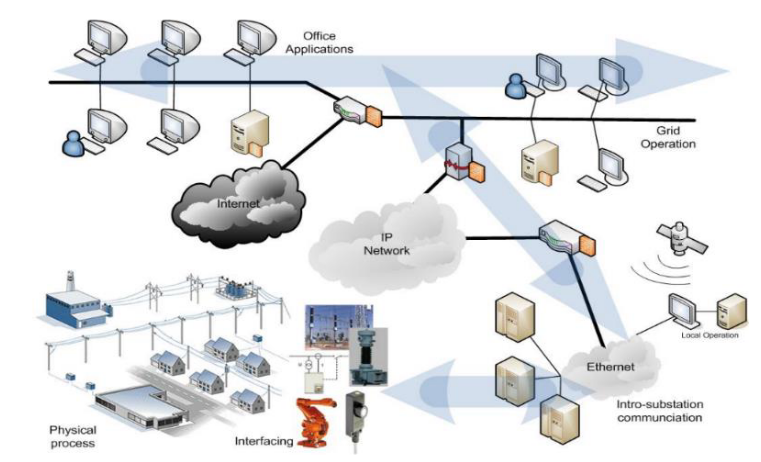
\includegraphics[width=0.8\textwidth, keepaspectratio]{ch2/assets/SAS.png}
	\caption{Design of Substation Automation Systems(Image credits: KTH, "Lecture 5: Substation Automation Systems")}
	\label{fig:substation-automation}
\end{figure}
%\FloatBarrier

\section{Backyard System}
The backyard system serves as the hub for all high-power apparatus, responsible for channeling energy from the power plant and facilitating its delivery to homes. It encompasses a range of critical devices, such as high-voltage circuit breakers, switches, voltage transformers for protection and measurement, current transformers for protection and measurement, high-voltage power transformers, capacitor banks, reactors, and synchronous compensators, devices that have gained increasing prominence in recent times. However, let's delve into the components found in any substation, as they will be detailed in the subsequent subsections.

\subsection{Circuit Breakers}
High-voltage circuit breakers play a crucial role in the operation and protection of electrical networks at very high, high, and medium voltages. They are electromechanical devices designed to interrupt the flow of electric current under abnormal conditions in the electrical network, such as short circuits and overloads. In the event of a network fault, the circuit breaker receives a signal from the electrical protection system detecting abnormalities. With this signal, the circuit breaker contacts quickly open to interrupt the electric current and extinguish the electrical arc generated when the contacts open, preventing damage to the network equipment.

Circuit breakers ensure the reliability of electrical power supply, with a focus on making electricity available to the entire network. High-voltage and very high-voltage circuit breakers are responsible for isolating detected faults in the system, preventing the spread of the defect to other parts of the network and thus avoiding widespread blackouts.

\subsection{Switches}
High-voltage switches play a pivotal role in the seamless operation of electrical networks at very high, high, and medium voltages. These electromechanical devices are intricately designed to isolate a section of the electrical system during normal operating conditions. When conducting maintenance on the electrical network, the switch opens a specific circuit segment, necessary for the safe and efficient execution of maintenance tasks. This ensures the well-being of maintenance personnel while simultaneously preserving the continuous operation of the electrical network.

In essence, very high, high, and medium voltage switches serve as integral components in power substations, offering a secure and dependable method for isolating designated sections of the electrical system. This isolation is essential for the maintenance of power system equipment, including transformers, circuit breakers, and capacitor banks. Importantly, this isolation process does not compromise the overall functionality of the substation(~\cite{janne2013switchgear}).

\subsection{Voltage Transformers}
Voltage transformers play a critical role in electrical systems by providing precise voltage measurements for each phase of the circuit. Their primary function is to convert very high voltages into more manageable, general-purpose voltages like 110V. The utilization of lower voltages facilitates easier handling, both in terms of magnitude and the insulation required for compatibility with IEDs.

Ensuring optimal signal quality is a key responsibility of voltage transformers. Their primary objective is to accurately replicate the high voltage in a lower voltage format, creating a precise replica with reduced values. This replication process is essential for utilizing the information in electrical protection, enabling the analysis of network disturbances, and facilitating timely action in the event of a fault.


\subsection{Current Transformers}
Current transformers play a crucial role in electrical systems, offering precise current measurements for each phase of the circuit. Their primary function is to convert very high currents into more manageable, general-purpose currents, typically around 1A. This reduction in current values enhances ease of handling, both in terms of magnitude and the insulation required for compatibility with IEDs.

Ensuring optimal signal quality is a paramount responsibility of current transformers. Their principal objective is to accurately replicate the high current in a lower current format, creating a precise duplicate with reduced values. This replication process is vital for utilizing information in electrical protection, enabling the analysis of network disturbances, and facilitating prompt action in the event of a fault.

\section{Intelligent Electronic Devices}
The IED formed by the set of units for data acquisition, processing, and transmission, located in substations, is generically referred to as a Remote Terminal Unit (RTU). At a given moment, it represented a significant evolution within a sector known for its conservatism in adopting new technologies, allowing remote control of substations by a central-level system, initiating the evolution of data transmission capacity through advances in telecommunications and the application of computers on a large scale. This enabled the expansion of the potential use of digital technology as a reality in substation environments(~\cite{NormaIEC61850}).

With consolidated digital electronics technology, the first proposals for Integrated Protection and Control Systems emerged, using protection relays and control units based on microprocessors and memories, with intelligence at the equipment level for logic execution and automation, introducing the concept of IED. These devices enable the use of computer networks for communication via fiber optics between terminals and relays within the same substation. In addition, personal computers are used at the control and monitoring level of the substation (~\cite{NormaIEC61850}).

\subsection{Protection Alghorithm System}
Protection stands as one of the paramount functions within a substation or any power system. Its primary goal is to ensure the safeguarding of equipment and personnel, while also minimizing damage in the event of electrical faults, short circuits, or overloads. This critical function is inherently local, designed to operate independently if necessary, irrespective of the substation's automation system. Even though it seamlessly integrates into the automation system under normal conditions, the integrity and effectiveness of protection functions should never be compromised or restricted within any power system automation (~\cite{NormaIEC61850}).

\subsection{Control System}
Local control involves autonomous control actions that a device can independently perform, such as interlocks, switching sequences, synchronism verification, and others. In this context, human intervention is limited, and the risks of errors are minimized. Similar to protection, local control should continue to operate even if the automation system is compromised.

Remote control functions are related to substation control executed by SCADA software. Commands can be directly issued to devices managed remotely, such as opening or closing a circuit breaker. Relay settings can be adjusted either through the device itself or a computer equipped with manufacturer-specific software. Additionally, desired information can be collected from protection relays using the IEC~61850 protocol via the MMS protocol. This eliminates the need for human actions within the substation to perform switching operations, making these actions faster. Furthermore, the SCADA terminal provides an overview of the entire plant, offering insights into ongoing activities and status (~\cite{NormaIEC61850}).

\subsection{Measurement}

A range of information from a substation is collected and analyzed in real-time by the automation system for its proper functioning. The measurement system consists of:

\begin{itemize}
	\item Electrical Measurements - voltages, currents, power, power factor, harmonics, etc;
	\item Monitoring Measurements of Equipment - such as transformer and motor temperatures;
	\item Disturbance Recorder - Recordings of disturbances for fault analysis.
\end{itemize}

This vast amount of information can assist in studies such as load flow analysis and planning for disturbances, in addition to being essential for protection and control functions (~\cite{NormaIEC61850}).

\subsection{Monitoring}
It is a sequence of events or part of the automation system with information that allows monitoring the state of the substation, such as equipment status, maintenance alerts, relay configurations, etc. This improves the overall system efficiency, enhancing the effectiveness of protection and control. These pieces of information are useful in fault analysis, determining what happened, when, where, and how it happened (location, time, and sequence)(~\cite{NormaIEC61850}).

\subsection{Communication Protocols}
The significant progress in substation automation has led to substantial investments by major IED manufacturers aiming to provide differentiation in protection and control equipment for substations. This competition has also given rise to a large number of proprietary communication protocols, which, to some extent, generated undesirable results in terms of interoperability. Substations with a large number of IEDs are highly likely to have undergone growth, with the current topology not being the original one. In such cases, equipment from different manufacturers is often present, and when connected to a single network, they do not communicate as expected in the vast majority of cases.

Faced with the communication challenges between devices, standardized protocols have emerged with the goal of achieving the desired interoperability. In other words, these protocols aim to enable communication between devices from different manufacturers on the same network. Figure~\ref{fig:table-protocols} displays some of the most commonly used protocols in substation networks (~\cite{NormaIEC61850}).

\begin{table}[h]
	\centering
	\scriptsize
	\resizebox{\textwidth}{!}{
		\begin{tabular}{@{}lcccc@{}}
			\toprule
			\textbf{Protocol} & \textbf{Originally used by} & \textbf{Speed} & \textbf{Access Principle} & \textbf{OSI Layers} \\ \midrule
			MODBUS                      & Gould-Modicon                    & 19.2 kbps           & Cyclic scanning             & 1, 2, 7              \\
			SPABUS                      & ABB (exclusive)                  & 19.2 kbps           & Cyclic scanning             & 1, 2, 7              \\
			DNP3.0                      & GE-Harris                        & 19.2 kbps           & Cyclic scanning\textsuperscript{2}            & 1, 2, 7\textsuperscript{3}             \\
			IEC 60870-5                 & All manufacturers                & 19.2 kbps           & Cyclic scanning             & 1, 2, 7              \\
			MODBUS+                     & Gould-Modicon                    & Token               & Cyclic scanning             & 1, 2, 7              \\
			PROFIBUS                    & Siemens                          & 12 Mbps             & Token                        & 1, 2, 7              \\
			MVB                         & ABB                              & 1.5 Mbps            & TDM                          & 1, 2, 7\textsuperscript{4}             \\
			FIP                         & Merlin-Gerin                     & 2.5 Mbps            & TDM                          & 1, 2, 7              \\
			Ethernet + TCP/IP           & All manufacturers                & 10 Mbps             & CSMA/CD                      & 1-7                  \\
			LON                         & ABB (exclusive)                  & 1.25 Mbps           & PCMSA/CD                     & 1-7                  \\
			UCA 2.0                     & GE                               & 10 Mbps             & CSMA/CD                      & 1-7                  \\ \bottomrule
		\end{tabular}
	}
	\caption{Communication Protocols used by energy company.}
	\label{table:protocols}
\end{table}



\section{Overview of IEC~61850}
IEC 61850 is an international standard for communication in substations and power utility automation. It defines a set of protocols and data models to enable the interoperability of devices within a substation, facilitating efficient and standardized communication for protection, control, monitoring, and automation purposes. Key features of IEC 61850 include:

\begin{itemize}
	\item Data Modeling: The standard introduces a standardized way of modeling substation data, using a hierarchical structure known as the Common Information Model (CIM). This allows for consistent representation of information across different devices.
	\item Communication Protocols: IEC 61850 specifies communication protocols for substation automation, with an emphasis on Ethernet-based communication. It defines how devices such as protection relays, controllers, and meters exchange information using protocols like MMS and GOOSE.
	\item Sampled Values: Part 9 of the standard, IEC 61850-9, introduces Sampled Values, enabling the transmission of digitized analog values, such as voltages and currents, in a standardized manner. This is crucial for real-time protection applications.
	\item Configuration Language: IEC 61850 includes SCL (Substation Configuration Language), a standardized language for describing the configuration of devices and systems within a substation. SCL allows for the exchange of configuration information between different devices.
	\item GOOSE Messaging: GOOSE messaging is a key feature that allows devices to exchange critical information in a peer-to-peer manner, enabling faster and more deterministic communication for protection and control functions.
	\item Interoperability: The standard aims to improve interoperability between devices from different manufacturers, promoting vendor-neutral solutions and reducing integration efforts in substations.
	\item Engineering Process: IEC 61850 defines an engineering process that standardizes the design, configuration, and testing of substation automation systems. This helps ensure consistency and reliability in the deployment of automation solutions.
\end{itemize}

IEC 61850 plays a vital role in modern and optimal power systems by provide a standardized framework for communication and automation in substations. It enhances reliability, flexibility, and interoperability in the evolving field of power utility automation.

\subsection{IEC 61850-1 - Introduction and Overview}

This initial segment provides a comprehensive introduction to the entire IEC 61850 series, offering a foundational framework for communication within substations. It sets the stage for subsequent standards, establishing a cohesive context for the standardization of communication in substation automation systems (~\cite{Overview_of_IEC_61850_and_Benefits}).

\subsection{IEC 61850-2 - Glossary}

Part 2 of the standard IEC61850, meticulously defines the glossary of terms used throughout the IEC 61850 series. By ensuring a uniform understanding of terminology, this section fosters clear communication and interpretation of the standards among diverse stakeholders in the energy sector (~\cite{Overview_of_IEC_61850_and_Benefits}).

\subsection{IEC 61850-3 - General Requirement}

This section outlines overarching requirements for communication networks and systems in substations. Covering aspects such as performance, testing procedures, and documentation standards, it provides a robust set of guidelines for the effective implementation of IEC 61850 (~\cite{Overview_of_IEC_61850_and_Benefits}).

\subsection{IEC 61850-4 - System and Project Management}

Centered on system and project management, this section provides valuable guidance for the seamless orchestration of IEC 61850 within substation communication systems. It encompasses essential aspects of planning, execution, and documentation, contributing to the successful deployment of the standard (~\cite{Overview_of_IEC_61850_and_Benefits}).

\subsection{IEC 61850-5 - Communication Requirements for Functions and Device Models}

Part 5 plays a pivotal role by defining communication profiles for specific functions and device models in substations. This ensures seamless interoperability between devices from different manufacturers, facilitating their integration within substation automation systems (~\cite{Overview_of_IEC_61850_and_Benefits}).

\subsection{IEC 61850-6 - Configuration Language for Communication in Electrical Substations}

This segment specifies a standardized language for articulating the configuration of communication in electrical substations, particularly in relation to IEDs. It streamlines the configuration process, enhancing consistency across diverge implementations(~\cite{Overview_of_IEC_61850_and_Benefits}).

\subsection{IEC 61850-7 - Basic Communication Structure}

Establishing the fundamental communication structure for substation and feeder equipment, Part 7 provides a foundational framework. It defines essential elements necessary for communication within substations, fostering a standardized structure for various devices (~\cite{Overview_of_IEC_61850_and_Benefits}).

\subsection{IEC 61850-8 - Specific Communication Service Mapping}

Part 8 concentrates on Specific Communication Service Mappings (SCSM), offering guidance for mapping diverse protocols used in substation communication. This ensures compatibility and smooth interaction between devices employing different communication protocols (~\cite{Overview_of_IEC_61850_and_Benefits}).

\subsection{IEC 61850-9 - Specific Communication Service Mapping}
Part 9 specifically deals with defining SCSM tailored for diverse protocols used in substation communication. It establishes a standardized framework to ensure compatibility and seamless interaction among different devices within substation automation systems. IEC 61850-9 is crucial for promoting interoperability and facilitating efficient communication among IEDs in substations by addressing the intricacies of various network layers (~\cite{Overview_of_IEC_61850_and_Benefits}).

\subsection{IEC 61850-10 - Conformance Testing}

Focusing on conformance testing, Part 10 establishes rigorous procedures and requirements to verify that devices and systems adhere to the IEC 61850 standard. This contributes to the reliability and compatibility of implementations by ensuring strict compliance through thorough testing processes (~\cite{Overview_of_IEC_61850_and_Benefits}).

\section{IEC 61850-9-2 Sampled Values (SV)}

This section discusses the evolution of the IEC 61850-9-2 protocols, tracing its development from its precursor in 2002, IEC 60044, to its current version, IEC 61850-9-2 Ed2, finalized in 2020.

\subsection{IEC 60044-8/2002}

Many in the industry are familiar with the IEC 60044 standard, a predecessor to the current IEC 61869 standard for instrument transformers. Part 8 of IEC 60044, dealing with electronic instrument transformers, introduced the concept of a "merging unit." This unit acts as a bridge between analog and digital signals, facilitating the conversion of analog network signals for use in digital IEDs. Additionally, the standard introduced the idea of a data set, later utilized in IEC 61850 for network communication.

Figure~\ref{fig:Merging-Unit} The concept of the MU represents the integration of various sensor data, such as current and voltage measurements, into a single digital output, streamlining communication between equipment and control systems. This concept laid the foundation for the development of the MUs available in the market today. The initial integration and design of MUs introduced a unified approach to handling data, which has since evolved into a critical component for ensuring efficient, reliable, and accurate data transmission in substations. \footnote{\url{https://www.linkedin.com/pulse/history-iec-61850-sampled-values-tibor-congo/}}

\begin{figure}[tbh]
	\centering
	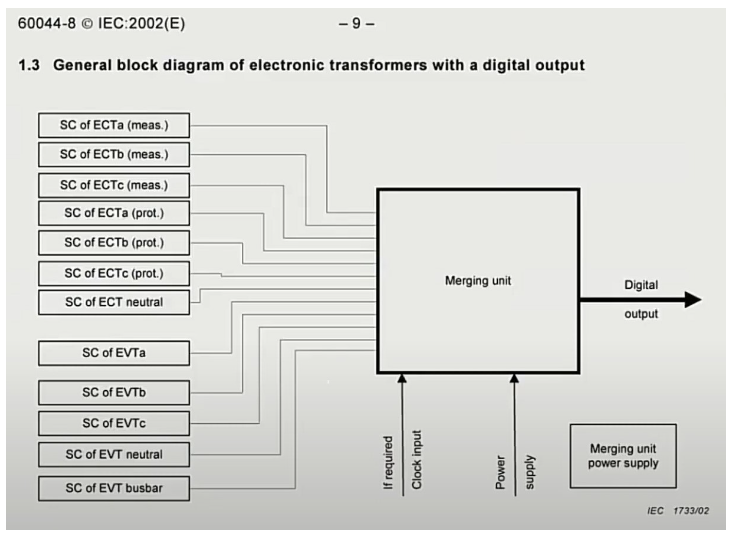
\includegraphics[width=\textwidth, keepaspectratio]{ch2/assets/Idea_of_Merging_Unit.png}
	\caption{Concept of the Merging Unit.}
	\label{fig:Merging-Unit}
\end{figure}
%\FloatBarrier

\subsection{IEC~61850-9-1/2003}

This marks the beginning of the protocol known today. However, it initially leaned towards a point-to-point communication model, resembling its predecessor IEC 60044. This approach lacked considerations for network applications, crucial for the interoperability that the protocol now provides. The concept of the Process Bus network, prevalent today, was not present during this period, causing delays in releasing the next version (~\cite{History_Sample_Value}).

\subsection{IEC~61850-9-2(Ed1)/2004}

At this stage, the abstraction of the IEC 61850 standard is being carefully applied once more. Initially introduced in the IEC 61850-7-2 standard, this service specification has since developed into a well-defined standard within IEC 61850-9-2, where it is clearly outlined within the context of Ethernet communication.

The data structure is characterized by its generic definition, and the communication process operates entirely independently. This implies that, in the future, we could seamlessly transition to another standard beyond Ethernet, tailored to the system's evolving needs. This flexibility is a testament to the power that abstraction brings. However, it's important to note that, thus far, the Ethernet protocol has been utilized and has consistently met the expected performance requirements.

In this revised standard, the noteworthy inclusion is the implementation of the process bus for Sampled Values, signaling a departure from the initial point-to-point communication approach. Here, to propagate Ethernet packets across the network, it leverages the existing multicast definition of the Ethernet protocol.

A widely embraced guideline employed by manufacturers in the development of Sampled Values is the UCA Implementation Guideline for IEC 61850-9-2.. It's crucial to recognize that this is a guideline, not a standard(~\cite{History_Sample_Value}).

\subsection{IEC 61850-9-2 Ed2/2011}

In this new edition, there were not many changes, mainly due to the fact that the energy industry was not significantly progressing in the adoption of this technology, even with lighter versions like IEC~61850-9-2-LE. The reasons for this lack of progress are attributed to the skeptical nature of many protection engineers. They tend to be more conservative when it comes to supplying electrical power, sometimes justified by negative experiences in the field(~\cite{History_Sample_Value}).

There were also some technical issues with SVs due to time synchronization. At that time, the most used protocol was SNTP, which allowed only millisecond precision. For SVs, higher precision in samples was needed. Additionally, there was immaturity in redundancy solutions in the network. Consequently, these two significant problems were only resolved later with the implementation of the following technologies:

\begin{itemize}
	\item Time Synchronization - Precision Time Protocol (PTP): This protocol enables time synchronization via Ethernet with a timing error of less than 1 microsecond. Synchronization could now be achieved through the Ethernet network connection, eliminating the need for a separate network for time synchronization of merging units in the field.
	\item Redundancy - Parallel Redundancy Protocol (PRP): PRP operates with effectively two duplicated networks, resembling the approach adopted by service providers in the transmission of electrical energy networks. These providers often maintain redundant protection/control systems. The loss of service in one of these networks does not compromise functionality, as the parallel network continues to perform its communication functions without affecting the protection/control systems.
	\item High Availability Continuous Redundancy (HSR): HSR provides redundancy through a ring architecture. This is essentially the same ring architecture, where communication service continuity is maintained through the open ring, in case of service loss in any part of the closed ring. In both cases, specific hardware (and software) requirements must be met to consider the implementation of the solution. This is a fundamental element in the design of the Digital Substation.
\end{itemize}

For time synchronization, the adopted solution was the Precision Time Protocol (PTP). With a resolution below 1 microsecond, this was sufficient for SVs to be synchronized, making it possible to reconstruct the digital waveform into analog again and check for faults or network issues by IEDs. In terms of redundancy, two solutions were implemented: PRP and HSR, with PRP being the more widely used due to lower associated implementation costs and the assurance of redundancy(~\cite{History_Sample_Value}).

\subsection{IEC 61869-9/2016}

The IEC 61869-9 standard is familiar to everyone using instrument transformers for other applications in the industry. This standard provided recommendations for measuring instruments, ranging from light versions to more demanding ones. The Figure~\ref{fig:SV-Tables} below summarizes this information.~\footnote{\url{https://www.linkedin.com/pulse/history-iec-61850-sampled-values-tibor-congo/}}

\begin{figure}[tbh]
	\centering
	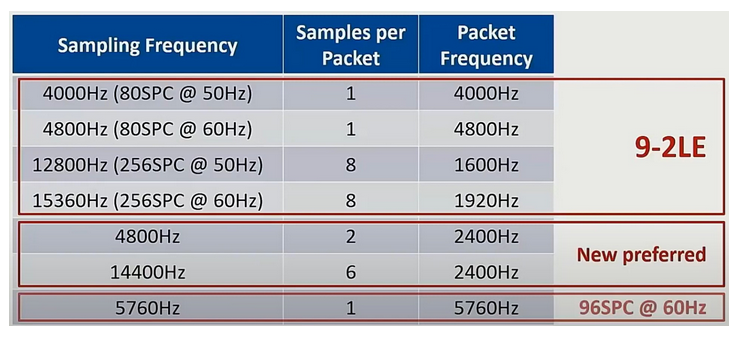
\includegraphics[width=\textwidth, keepaspectratio]{ch2/assets/table_SVs_Frequency.png}
	\caption{Frequency regarding Sampled Values.}
	\label{fig:SV-Tables}
\end{figure}
%\FloatBarrier

The information derived from the table indicates that protection functions use a sampling rate of 4800Hz at 60Hz and 4000Hz at 50Hz according to the IEC~61850-9-2-LE version. When we talk about preferred streams, the sampling rates remain the same regardless of their use, such as protection, measurement, or power quality. This balance is achieved by adjusting the necessary samples per Application Specific Data Unit (ASDUs) per packet.

The IEC61869-9 standard mentions the use of configurable datasets. The IEC 61850-9-2-LE version simplified this by publishing 4 currents + 4 voltages for all datasets. While this approach was efficient, it lacked flexibility. Therefore, IEC61869-9 introduces flexibility in this regard, optimizing the implementation. However, this increased flexibility also brings greater complexity to data processing(~\cite{History_Sample_Value}).

\subsection{IEC~61850-9-2 Ed2.1/2020}

In this latest update, there was a small reinforcement of what was mentioned in the previous version. Here, a new field called SynchSrcID was introduced, which is used to specify the synchronization source of the merging unit. This new feature is one of the optional fields. In the IEC~61850-9-2-LE version, there was only one field, but breaking free from the limitations of this version, now there are more fields to configure. Again, a note on what was mentioned above, it is essential to analyze configuration issues and implementation costs, as it will be more complex(~\cite{History_Sample_Value}).\newline


The evolution from IEC 60044-8 to IEC 61850-9-2 ED2.1 marks the shift from analog to digital in substation communication. Starting with the digitization of transformer outputs, it progressed through increasingly sophisticated standards (IEC 61850-9-1, 9-2 ED1, and 9-2 LE), refining the transmission of sampled values over Ethernet. The development culminated in IEC 61869-9 and IEC 61850-9-2 ED2.1, which ensure interoperability and advanced digital communication in modern substations, in Figure~\ref{fig:Evolution of IEC 61850-9-2} ~\footnote{\url{https://www.linkedin.com/pulse/history-iec-61850-sampled-values-tibor-congo/}} has showned the progress through years.

\begin{figure}[tbh]
	\centering
	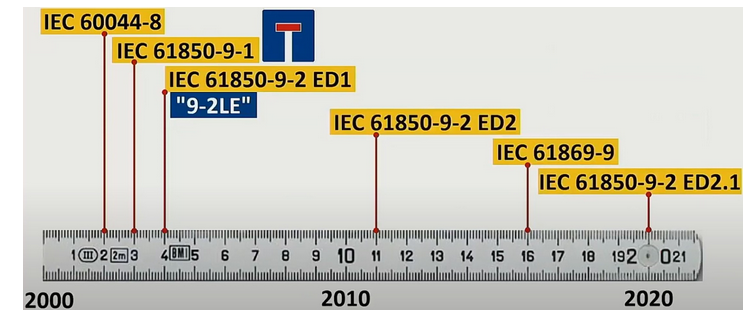
\includegraphics[width=\textwidth, keepaspectratio]{ch2/assets/evolucao_SV_protocol.png}
	\caption{Evolution of IEC 61850-9-2}
	\label{fig:Evolution of IEC 61850-9-2}
\end{figure}


%\FloatBarrier

% Chapter 3
\chapter{Analysis and Design of the Solution} % Main c%----------------------------------------------------------------------------------------

\section{Description of Equipment and Functions}

This work focuses on the equipment configuration within an electrical substation following the IEC 61850 standard, specifically addressing MUs and their role in substation automation. Merging Units are responsible for converting analog signals from current transformers and voltage transformers into digital data, known as sampled values, which are then transmitted to protection relays. These relays ensure the safe operation of the electrical grid by monitoring data and acting on potential faults.

In the system studied, two MUs are connected to the same CTs and VTs, providing redundant SV streams to the protection relays. This redundancy ensures continuous operation, even if one MU fails, as the other can still deliver accurate data. However, this dual-stream configuration poses a challenge: the protection relay must decide which of the two SVs to use for executing protection algorithms. These algorithms detect anomalies or faults in the grid, so selecting the most reliable SV is crucial for maintaining system performance and safety.

In the current setup, the protection relay passively receives SVs from both MUs, with no dynamic mechanism in place to prioritize or select the best sample in real-time. This can lead to inefficiencies or even errors if the data from one MU is compromised.

\section{Limitations of the Current Solution}

The primary limitation of the existing system is the lack of an algorithm that dynamically selects the best SV from the multiple streams sent by the MUs. Without this, the protection relay may process suboptimal or even erroneous data, especially in cases where one MU is malfunctioning or sending corrupted SVs. This limitation is critical, as the protection relay’s decisions directly impact the safety and reliability of the substation.

Moreover, the current system does not fully exploit the redundancy provided by the MUs. Although two SV streams are available, the relay does not have a built-in method to evaluate the quality of these samples and select the most reliable one. This absence of real-time evaluation increases the risk of incorrect fault detection, which could compromise the protection system's integrity.

\section{Proposed Solution}

To address the limitations identified, we propose an algorithm designed to dynamically evaluate and select the most reliable SV from multiple streams sent by the MUs. This solution acts as an intelligent selector that monitors the incoming SVs, assesses their quality, and ensures that only the most accurate and reliable sample is used in protection calculations.

\subsection{SV Selection Algorithm}

The algorithm continuously monitors SVs arriving from two MUs connected to the same CTs and VTs. It evaluates these samples based on predefined quality metrics, such as accuracy, transmission latency, and packet integrity. Once the evaluation is complete, the algorithm selects the SV with the best overall performance, allowing the protection relay to process only the most reliable data.

This approach ensures that even in the event of a partial MU failure, the protection relay will continue to operate with accurate data. By dynamically selecting the best SV, the algorithm mitigates the risk of using unreliable or corrupted data, thus enhancing the reliability of the entire protection system.

\subsection{Operational Flow of the Algorithm}

The algorithm operates like a switch, receiving two or more SV streams from the same sensor (CT or VT) and passing only the best sample to the protection relay. The selection process involves the following steps:
\begin{itemize}
	\item Data Monitoring: The algorithm receives SVs from both MUs and continuously monitors the quality of each stream.
	\item Classification: The SVs are classified based on criteria such as latency, accuracy, and error detection.
	\item Selection: The sample with the highest classification is selected, while the other is discarded.
	\item Protection Execution: The protection relay uses the selected SV to run fault detection algorithms.
\end{itemize}

This process repeats at each cycle, ensuring that the protection system operates with the most reliable data at all times. Figure~\ref{fig:SLD_Diagram}~\footnote{\url{https://www.efacec.pt/en/wp-content/uploads/2022/08/CS491I2207A1_MCU-500.pdf}} illustrates a simplified single-line diagram (SLD) of a substation using this architecture, showing the relationship between MUs and the protection relay.

\begin{figure}[tbh]
	\centering
	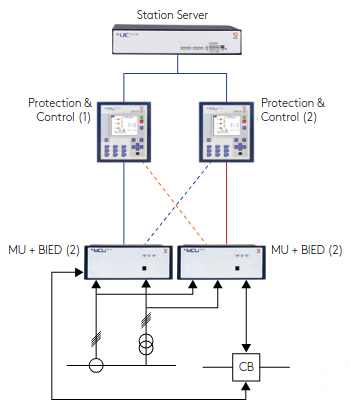
\includegraphics[width=0.77\textwidth, keepaspectratio]{ch3/assets/SLD_Diagram.png}
	\caption{Simple Single Line Diagram (SLD) of an Electrical Substation with SV streams. (Source: Efacec Energia, Máquinas e Equipamentos Eléctricos, S.A.)}
	\label{fig:SLD_Diagram}
\end{figure}

\subsection{Handling Redundancy and Failures}

The proposed solution efficiently manages redundancy by ensuring that the relay always uses the best available data. If one MU fails or its SV stream becomes unreliable, the algorithm automatically switches to the stream with the highest quality, maintaining uninterrupted and accurate protection relay operation. This dynamic handling of redundancy adds an extra layer of resilience to the protection system, preventing erroneous detections and unnecessary interruptions in service.

\section{Conclusion}

In this chapter, we first outlined the configuration and roles of the MUs and protection relays in the substation, explaining how they operate within the context of IEC 61850. We then highlighted the limitations of the current system, particularly the absence of an effective mechanism for selecting the best SV from multiple MUs. Finally, we introduced the architecture of a novel algorithm that dynamically selects the most reliable SV, ensuring higher accuracy and reliability in protection relay operations.

% Chapter 4

\chapter{Architecture} % Main chapter title

\label{chap:Chapter4} % For referencing the chapter elsewhere, use \ref{chap:Chapter4} 

%----------------------------------------------------------------------------------------

This chapter details on the practical implementation of the proposed algorithm. It begins with an overview in Section 4.1, which outlines the key methods and tools used throughout the development process. Section 4.2 dives into the detailed steps taken to develop the algorithm, including both hardware and software components, as well as the various tools and libraries (crates) employed. Section 4.3 then describes the algorithm designed to select the best SVs and presents the results of this selection process. This chapter provides a comprehensive view of how the theoretical concepts were translated into a working solution.

\section{Overview}

The demand for an algorithm that selects the optimal analog signal has grown alongside the increasing adoption of merging units in substations. As substations transition to digitalization, merging units become indispensable for ensuring efficient performance. These units play a critical role by making various other substation components dependent on their technology. Previously, the only critical protocol was GOOSE, used for transmitting trip signals and equipment interlocks. Now, with the adoption of merging units, the communication network itself becomes critical. It ensures the accurate reception of analog signals from CTs and VTs, allowing protection algorithms to promptly identify network faults.

Consequently, formerly non-critical equipment like switches must now meet stringent performance criteria to prevent delays. This necessitates the implementation of PTP across all critical network devices, establishing PTP as the master clock for the entire substation network.

Merging units are ushering substations into the digital age, yet they also introduce new challenges. In older substations, concerns about analog signals were limited to issues like broken wires and induction. Today, with numerous interconnected devices requiring precise timing and high performance, ensuring proper system operation becomes crucial.

\section{Hardware Setup}

For the development and execution of this project, a Dell Inspiron personal computer has been utilized. This machine is equipped with robust specifications to support the complex computational and networking requirements of the research. The key features of this computer are as follows:

\begin{itemize}
	\item Processor: Intel Core i5 10th Generation, offering a balanced blend of performance and efficiency for handling various computational tasks required during the development and testing phases.
	\item Memory: 8 GB of RAM, providing sufficient memory capacity to run multiple applications and perform intensive data processing operations seamlessly.
	\item Networking: The system includes two Ethernet cards to facilitate network connectivity:
	Integrated Ethernet Card: The built-in Ethernet card that comes with the computer.
	Gigabit USB to Ethernet Adapter: An additional gigabit Ethernet adapter connected via USB, enhancing the computer’s networking capabilities.
	Network Speed Limitation: Despite the presence of a gigabit Ethernet adapter, the overall system network speed is limited to 100 Mbits/s. This is due to the maximum speed supported by the jetson nano, which is being used in conjunction with the Dell Inspiron for this project.
\end{itemize} 

The Jetson Nano stands out for its versatility and compact design, making it an ideal choice for deploying sophisticated algorithms in research projects. Key features include:

\begin{itemize}
	\item Processing Power: Equipped with a 1.43 GHz quad-core ARM Cortex-A57 processor and a 128-core NVIDIA Maxwell GPU, offering robust computational capabilities necessary for real-time data processing and algorithm execution.
	\item Memory: Includes 4 GB of LPDDR4 RAM, ensuring efficient storage and retrieval of data crucial for running complex algorithms and maintaining system responsiveness.
	\item Connectivity: Integrated with Gigabit Ethernet, enabling high-speed wired communication essential for modern substation automation applications, and also an ethernet adapter using USB3.0 with gigabit connection.
	\item GPIO Pins: Equipped with a 40-pin GPIO header, allowing direct interfacing with external sensors, actuators, and other peripherals, which is indispensable for hardware integration in substation environments.
\end{itemize}

The specifications of the Dell Inspiron ensure it can manage the comprehensive demands of the research, ranging from the development and testing of algorithms to interfacing with the Jetson Nano for real-time data processing and network simulations. Equipped with an Intel Core i5 10th Generation processor and 8 GB of RAM, this personal computer provides the necessary performance and memory capacity for running complex applications and intensive data operations. The inclusion of dual Ethernet cards—one integrated and one gigabit USB to Ethernet adapter—enables flexible and reliable network configurations, essential for accurately emulating substation environments and conducting thorough testing.

The Jetson Nano is equally well-suited for executing the algorithm designed to optimize SV selection in substation automation systems. Its powerful ARM processor and NVIDIA GPU offer robust computational capabilities and efficient data handling. The integrated Gigabit Ethernet facilitates high-speed wired communication, while the 40-pin GPIO header allows for direct interfacing with external sensors and actuators. Despite the network speed being limited to 100 Mbits/s due to the maximum capacity of certain interfaces, these features collectively ensure reliable performance and effective integration into research and development efforts.

By harnessing the strengths of both the Dell Inspiron and the Jetson Nano, this research project benefits from a synergistic blend of hardware capabilities. The Dell Inspiron serves as a robust foundation for development, testing, and executing the algorithm, leveraging its computational power and memory capacity. Meanwhile, the Jetson Nano operates as both a merging unit and a protection relay, demonstrating its adaptability and connectivity. This dual functionality makes the Jetson Nano an optimal platform for handling real-time data processing and network simulations. Together, these platforms play a pivotal role in advancing substation automation, improving operational efficiency, and bolstering the reliability of substation systems.

\section{Software Technologies}

The software development process began with selecting the programming language for developing the algorithm. Today, we have many languages that meet performance needs and are widely used in the market, such as C and C++. These languages prioritize performance, which is why they are predominantly used in embedded systems. However, we also have languages that are easier to develop and write, although not as performant, such as Python/MicroPython.

After thoroughly analyzing the scenario in which my development needed to be inserted, I came across the Rust language. Rust offers performance comparable to C and C++ but without the memory management issues inherent to these languages. Given that this development is related to critical systems, I opted to use a safer language. Thus, the development was carried out in Rust.

The decision to use Rust was also influenced by its modern design principles and strong community support. Rust’s ownership model ensures memory safety and eliminates common bugs such as null pointer dereferencing and buffer overflows. This is particularly important in critical systems where reliability and safety are essential.

Furthermore, Rust's rich type system and pattern matching capabilities facilitate the development of robust and maintainable code. The language's concurrency model is designed to prevent data races, making it a suitable choice for applications requiring high performance and safety.

By choosing Rust, the development process benefits from both high efficiency and enhanced safety, ensuring that the algorithm operates reliably within the substation automation system. This strategic choice underscores the commitment to using cutting-edge technologies to achieve optimal performance and reliability in critical system applications.

\subsection{Cargo}

Cargo is Rust's official package manager and build system, integral to managing Rust projects. It simplifies the process of managing dependencies, compiling code, running tests, and creating documentation. Here's an overview of Cargo's key features:

\begin{itemize}

	\item Dependency Management
	\begin{itemize}
		\item Crates: Cargo allows developers to easily include third-party libraries (known as crates) into their projects. These crates are listed in a Cargo.toml file, where you can specify the version of each dependency.
		\item Automatic Resolution: Cargo automatically fetches and compiles these dependencies, ensuring that the correct versions are used, and resolving any conflicts between different versions of the same crate.
	\end{itemize}

	\item Build and Compilation
	\begin{itemize}
		\item Automatic Resolution: Cargo automatically fetches and compiles these dependencies, ensuring that the correct versions are used, and resolving any conflicts between different versions of the same crate.
		\item Cross-Compilation: Cargo supports cross-compilation, allowing developers to build their Rust projects for different target platforms, which is particularly useful for embedded systems.
	\end{itemize}

	\item Project Management
	\begin{itemize}
		\item Project Initialization: Starting a new Rust project is simple with Cargo. By running cargo new 'project name', Cargo automatically creates a new directory with a basic Rust project structure, including the necessary Cargo.toml file and a default source directory.
		\item Workspaces: Cargo supports workspaces, enabling the management of multiple related packages within a single repository. This is particularly useful for large projects with multiple components that need to be developed and managed together.
	\end{itemize}

	\item Community and Ecosystem
	\begin{itemize}
		\item Crates.io: Cargo is tightly integrated with Crates.io, the Rust community's official crate registry. This allows developers to publish their libraries and applications, making them available to others in the community.
		\item Cargo.lock: Cargo manages a Cargo.lock file that records the exact versions of all dependencies used in a project, ensuring consistency across different builds and environments.
	\end{itemize}
\end{itemize}

Cargo's function in the Rust ecosystem is fundamental, as it provides a unified way to manage the entire lifecycle of a Rust project—from development and dependency management to testing, documentation, and deployment. Its user-friendly interface and powerful features make it an essential tool for Rust developers, facilitating a smooth and efficient development process.

\subsection{Crates}
Crates in Rust are the building blocks of Rust projects and packages. A "crate" refers to a compilation unit in Rust and can be a library or a binary.

\begin{itemize}
	
	\item Types of Crates
	\begin{itemize}
		\item Binary Crates: These are executable applications. When you create a binary crate, it generates a single executable file.
		\item Example: If you write a Rust program with a main.rs file, it’s a binary crate because it compiles to an executable.
		\item Library Crates: These contain reusable code that other projects can depend on. Instead of producing an executable, a library crate compiles to a .rlib file that other projects can link against.
		\item Example: A collection of utility functions or algorithms that you can share across multiple projects.
	\end{itemize}
	
	\item Crates.io
	\begin{itemize}
		\item Crates.io is the official Rust package registry where developers can publish and share their library crates. It's similar to npm for Node.js or PyPI for Python.
		\item Developers can search for and download crates published by others, integrating them into their projects with ease.
	\end{itemize}
	
	\item Dependency Management with Crates
	\begin{itemize}
		\item In Rust, projects can depend on other crates. You specify these dependencies in the Cargo.toml file, which lists all the crates your project needs, along with their versions.
		\item Cargo, Rust’s package manager, handles fetching these dependencies from Crates.io, ensuring compatibility and managing versions.
	\end{itemize}
	
	\item Benefits of using Crates
	\begin{itemize}
		\item Modularity: Crates encourage modular design, making it easy to split a project into smaller, reusable components. Each crate can be developed, tested, and compiled independently. needs, along with their versions.
		\item Reusability: By using crates, you can leverage existing solutions for common problems. Whether it's handling dates, parsing JSON, or working with databases, there’s likely a crate for it.
		\item Dependency Management: Cargo automatically manages dependencies, ensuring that you’re using the correct versions of the crates your project depends on, thus avoiding compatibility issues.
	\end{itemize}
	
	\item Community and Ecosystem
	\begin{itemize}
		\item The Rust community actively contributes to the ecosystem by publishing high-quality crates on Crates.io. This makes it easier for developers to find reliable, well-maintained packages for their projects.
	\end{itemize}
\end{itemize}

%In this project, I am exclusively using library crates, which are essential to the development process. These libraries significantly streamline the development work and provide crucial functionality. Additionally, by managing these libraries with Cargo, I can easily track and control the versions I’m using, ensuring consistency throughout the project.

This work relies exclusively on library crates, which are essential to the development process. These libraries significantly streamline the development work and provide crucial functionality. Additionally, managing these libraries with Cargo allows easy tracking and control of the versions being used, ensuring consistency throughout the project.

%Crates are central to the Rust ecosystem, promoting code reuse, modularity, and collaboration. Whether you’re building a small utility or a large-scale application, crates help structure your project and tap into the wealth of libraries and tools available in the Rust community. Below, I’ll describe the most important libraries that have been integral to this development.

Crates are central to the Rust ecosystem, promoting code reuse, modularity, and collaboration. Whether building a small utility or a large-scale application, crates help structure the project and tap into the wealth of libraries and tools available in the Rust community. Below, the most important libraries integral to this work are described.


\subsection{Tokio Crate}

Tokio\footnote{\url{https://crates.io/crates/tokio}} is one of the most popular and robust asynchronous runtimes in the Rust ecosystem, offering essential components for building high-performance, reliable, and scalable network applications. Leveraging Rust’s concurrency model, Tokio provides an event-driven, non-blocking I/O system that allows developers to handle thousands of concurrent connections with minimal overhead. This is particularly beneficial for applications that perform extensive I/O operations, such as reading from or writing to sockets, without needing to wait for these operations to complete before continuing with other tasks.

In addition to its asynchronous runtime, Tokio includes a comprehensive set of utilities such as timers, channels, and synchronization primitives, which are invaluable in managing complex concurrent systems. Its seamless integration with Rust's async/await syntax significantly simplifies the development of asynchronous code, making it more readable and maintainable.

A key feature of Tokio is its advanced multithreaded, work-stealing task scheduler, which is critical for optimizing the performance of asynchronous applications in Rust. This scheduler distributes tasks efficiently across multiple threads, ensuring full utilization of available CPU cores. By using a work-stealing approach, Tokio ensures that no single thread becomes a performance bottleneck. If one thread finishes its tasks while others are still occupied, it can "steal" tasks from the busy threads, leading to a more balanced and efficient distribution of workload.

This design is particularly beneficial in scenarios where an application must manage a large number of concurrent operations, such as handling network connections or processing real-time data streams. The scheduler minimizes idle time and maximizes throughput, which is essential for maintaining high-performance levels in demanding applications. Additionally, by automatically balancing the load, the scheduler reduces the need for manual optimization, allowing developers to concentrate on the core logic of their applications rather than focusing on performance tuning across threads. This makes Tokio an ideal choice for building scalable and responsive systems in Rust.

Tokio has to offer essential tools for managing concurrency and parallelism efficiently like:

\begin{itemize} 
	\item Concurrency and Parallelism: Tokio enables the handling of numerous tasks concurrently, facilitating the development of highly efficient and responsive applications. By utilizing asynchronous programming, Tokio helps manage multiple operations simultaneously without blocking the execution of other tasks. 
	\item Asynchronous I/O: Tokio excels in non-blocking I/O operations, making it ideal for applications that need to handle multiple network connections concurrently. This is particularly relevant for the merging unit and protection relay functions in this project. 
	\item Scalability: With Tokio, systems can scale efficiently, handling increased loads without a significant decline in performance. This is especially important for real-time data processing and network simulations required in substation automation systems.
\end{itemize}

By incorporating Rust and leveraging the Tokio crate, the development process benefits from high efficiency and enhanced safety, ensuring that the algorithm functions reliably within the substation automation system. This strategic choice highlights the commitment to using cutting-edge technologies to deliver optimal performance and reliability in critical system applications.

\subsection{Serde Crate}

Serde\footnote{\url{https://crates.io/crates/serde}} is the standard crate for serialization and deserialization in Rust, offering a flexible and highly efficient framework for converting complex data structures to and from various formats, such as JSON, TOML, YAML, and more. Serialization is the process of converting a data structure into a format that can be stored or transmitted, while deserialization is the reverse operation. Serde's performance is one of its standout features; it’s designed to minimize overhead and maximize speed, making it suitable for high-performance applications where data exchange is frequent and data structures are large or complex.

Serde ecosystem is extensive, with support for a wide range of data formats and seamless integration with other Rust crates. The framework is highly extensible, allowing developers to define custom serialization and deserialization logic for their data types. This flexibility ensures that Serde can handle nearly any data representation need, whether it's a simple JSON API or a complex, nested configuration file. Furthermore, Serde derive macros (\texttt{\#\textbackslash{}derive(Serialize, Deserialize)}) make it incredibly easy to implement serialization and deserialization for Rust structs and enums, saving developers from writing boilerplate code.

\subsection{Crc32Fast Crate}

Crc32Fast\footnote{\url{https://crates.io/crates/crc32fast}} is a high-performance crate designed to compute CRC-32 checksums efficiently. CRC-32 (Cyclic Redundancy Check) is a widely used algorithm for detecting errors in data transmission or storage. It’s a lightweight but powerful tool that can quickly determine if data has been corrupted, making it indispensable in contexts like file integrity checks, network communications, and data archival. The crc32fast crate is optimized for speed, using techniques like loop unrolling and SIMD (Single Instruction, Multiple Data) instructions to process data in parallel, significantly speeding up checksum computations.

This crate is particularly useful in applications where performance is critical, such as systems that handle large volumes of data or require real-time error detection. For example, in networking, CRC-32 checksums are often used to ensure that packets are received without errors. By integrating crc32fast into such a system, developers can maintain high throughput while ensuring data integrity. Additionally, its simplicity and efficiency make it a go-to choice for Rust developers needing a reliable method for error-checking large datasets or streams.

\subsection{Pnet Crate}

Pnet\footnote{\url{https://crates.io/crates/pnet}} (Packet Network) is a low-level networking crate in Rust that provides extensive capabilities for crafting, sending, and receiving raw network packets. It offers granular control over network communications, making it an essential tool for developers working on networking protocols, network security applications, or custom network infrastructure. Pnet allows you to build and dissect packets for various network layers (Ethernet, IP, TCP/UDP, etc.), giving you the ability to create highly customized network interactions that go beyond what standard networking libraries offer.

One of Pnet's key strengths is its flexibility. It supports a wide range of protocols and can be used for tasks like network monitoring, building packet sniffers, creating custom firewall rules, or even developing your own network protocol. Additionally, Pnet is well-integrated with Rust’s safety guarantees, meaning you can perform low-level network programming with fewer risks of common bugs, such as buffer overflows or memory leaks. This makes Pnet an excellent choice for developers who need both the power of low-level networking and the safety of Rust.

\subsection{Log Crate}

Log\footnote{\url{https://crates.io/crates/log}} is a logging facade for Rust that provides a simple and flexible way to capture log messages in your applications. It’s designed to be lightweight and minimal, focusing on defining a standard logging API that libraries and applications can use without committing to a specific logging implementation. This approach allows you to write code that logs messages at various levels (error, warn, info, debug, trace) and later decide how those logs are handled, whether they're printed to the console, written to a file, or sent to a logging service.

The log crate’s primary advantage is its decoupling of log producers from log consumers. You can use the log macros (log!, info!, error!, etc.) throughout your codebase, and then choose or implement a logging backend (like env\_logger or slog) that suits your application's needs. This flexibility makes log an ideal choice for libraries, as it allows the library to emit logs without enforcing a specific logging behavior on the end user. As a result, the log crate has become a standard in the Rust ecosystem, used by many libraries and applications to ensure consistent and configurable logging.

\subsection{Env\_Logger Crate}

Env Logger\footnote{\url{https://crates.io/crates/env_logger}} is a simple but powerful logging backend for the log crate, designed to configure logging via environment variables. This crate is particularly useful in situations where you need to adjust the verbosity of logging without modifying the code itself, such as in different deployment environments (development, testing, production). By setting environment variables, you can control which log levels are enabled and where the log output is directed, making env\_logger extremely flexible and easy to use.

For example, in a production environment, you might want to only log warnings and errors, while in a development environment, you might enable debug and trace logs to troubleshoot issues. Env\_logger supports these scenarios by allowing you to configure log levels on a per-module basis, providing granular control over the logging output. This makes it an invaluable tool for developers who need to maintain visibility into their applications’ behavior across different environments without cluttering the codebase with log configuration details.

\subsection{Chrono}

Chrono\footnote{\url{https://crates.io/crates/chrono}} is a comprehensive and robust date and time library for Rust, offering a rich set of features for working with dates, times, and time zones. It’s designed to be easy to use yet powerful enough to handle complex date and time manipulations. Chrono allows you to parse and format date/time strings, perform arithmetic operations on dates and times (e.g., adding or subtracting time durations), and work with time zones, including conversions between UTC and local times.

One of Chrono's most significant advantages is its flexibility and precision, making it suitable for a wide range of applications. Whether you need to manage timestamps in a database, schedule tasks, log events, or handle time-sensitive operations in a global application, Chrono provides the tools you need. It also supports custom date and time formats, allowing you to work with both standard and non-standard representations of time. Chrono is widely adopted in the Rust ecosystem for any application that requires accurate and reliable date/time handling.

\section{Solution Design}

This thesis proposes a method for selecting the best analog/digital signal sent by multiple Merging Units. The signal is initially analog because it is acquired in that form from VT and CT, but the Merging Unit converts it into a digital signal following the IEC-61850-9-2 protocol. The device proposed in this work receives the digital signal, compares it with another one that's come from another Merging Unit. After this comparison, an algorithm implemented using a state machine selects which signal will be forwarded to the protection systems subscribing to these SV.

To achieve this, it was necessary to develop and implement the IEC~61850-9-2 protocol from the ground up. Since there is no available library for the RUST programming language, one had to be created. As a result, a publisher, a subscriber, and the core algorithm which is the main focus of this thesis were developed. This algorithm must receive information from two Merging Units and, after processing it, send the selected data to the protection system.

Figure~\ref{fig:overview_of_implementation} The components of the thesis are interconnected as follows: Two MUs send data to the algorithm. The algorithm then evaluates the information from both MUs, selects the most optimal data, and transmits it to the Protection Relay. This selection process ensures that the Protection Relay receives the best possible data based on the criteria defined by the algorithm.

\begin{figure}[tbh!]
	\centering
	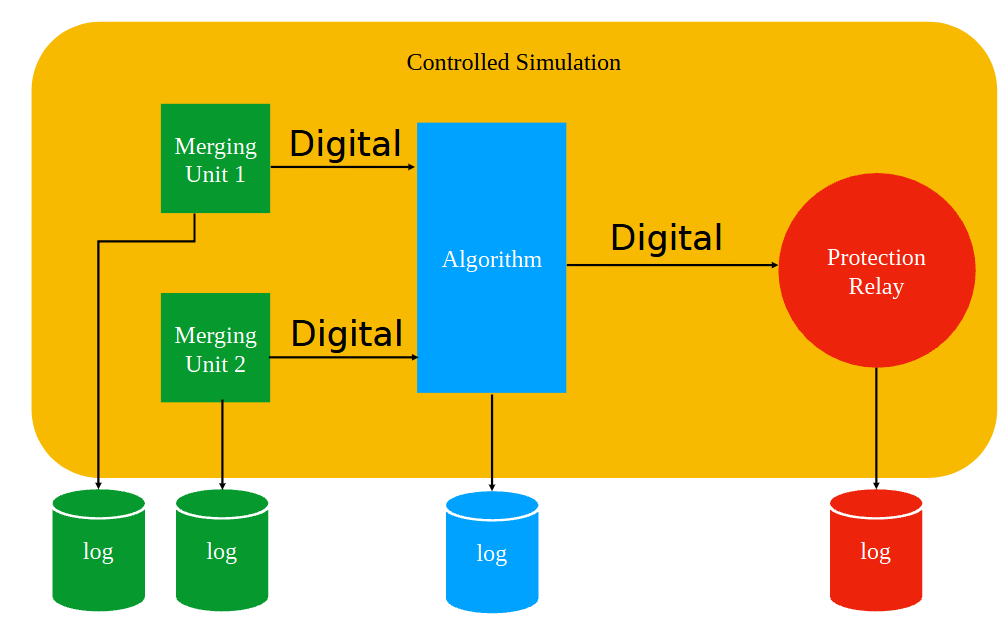
\includegraphics[width=0.80\textwidth, keepaspectratio]{ch4/assets/Implementation.png} % Reduce to 90% of the text width
	\caption{How the implementation was designed to work.}
	\label{fig:overview_of_implementation}
\end{figure}
%\FloatBarrier

%\raggedright
The development process began with the creation of the publisher, a software that emulates the operation of a Merging Unit. This software was built in accordance with the standard IEC~61850-9-2 for SV packets.

Figure~\ref{fig:sv_packet} shows the frame structure of a Sampled Value (SV) Packet~\footnote{\url{https://www.typhoon-hil.com/documentation/typhoon-hil-software-manual/References/iec_61850_sampled_values_protocol.html}}.

\begin{figure}[tbh!]
	\centering
	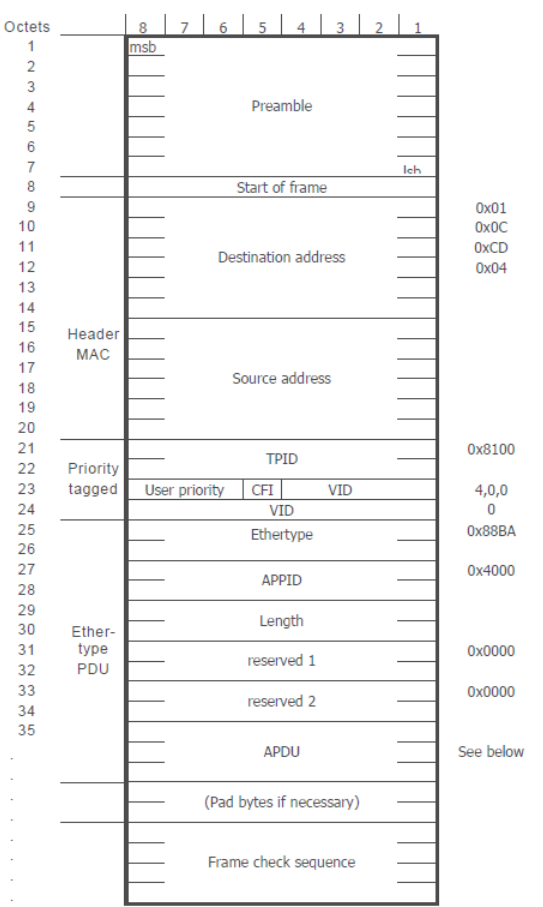
\includegraphics[width=0.75\textwidth, keepaspectratio]{ch4/assets/SV_Packtes.png} % Reduce to 90% of the text width
	\caption{How is constructed a Sampled Values Packet following the standard IEC~61850-9-2 (Image credits: Typhoon HIL)}
	\label{fig:sv_packet}
\end{figure}
%\FloatBarrier


Once the packet structure was defined, a function was created to calculate the values to be sent along with the SVs. This function uses the current execution time to generate similar values between the two Merging Units.

We also implemented verification and validation of the packets using Cyclic Redundancy Check (CRC). The CRC is added to the SV packet during its creation, and on the subscriber side, it is verified to ensure the packet's validity.

The second phase of development focused on the subscriber. Upon receiving the packet over the Ethernet network, and in compliance with the IEC~61850-9-2 protocol standards, the packet is reconstructed, its integrity validated using CRC, and the relevant information extracted and logged. The subscriber device we developed acts as a protection relay, where the received information is converted back to an analog signal and applied to the relay’s protection algorithms.

The third phase centered on developing the algorithm for selecting the best SV. This selection process involves analyzing the values received in the SV packets. To achieve this, we implemented an SV subscriber capable of retrieving data transmitted via this protocol, utilizing components from the earlier development stages. After receiving the data via Ethernet, the information is extracted, evaluated, and the best signal is chosen between the packets sent by Merging Unit 1 and Merging Unit 2. Once the best signal is identified, it is sent using the SV publisher, thus completing the development process aligned with the thesis's objectives.

The algorithm utilizes the Tokio crate, which provides a work-stealing task scheduler, allowing for concurrent and parallel processing. This enables the immediate retransmission of packets from the Merging Unit with the better signal, with the algorithm switching only when another Merging Unit provides a superior analog signal. This approach ensures real-time performance, essential for the required application.

This thesis specifically addresses scenarios involving two Merging Units. Although the case of more than two Merging Units was not considered, the algorithm can be adapted to handle such situations.
	
\section{Algorithm Description}

The description of the algorithm hinges on a deep understanding of both the publisher and subscriber functions. The aim is to create an algorithm capable of selecting the optimal samples from two independent devices that measure the same electrical quantity. This involves transmitting these measurements via a protocol, decompressing the data, extracting the necessary values, evaluating them, and ultimately selecting the best sample. All of this must be accomplished within a timeframe that ensures the SVs reach the protection devices without delay each SV being transmitted every 250 microseconds.

The algorithm is triggered upon the reception of an SV from one of the merging units. Once received, the SV is processed and evaluated to determine whether it is valid, invalid, or questionable. If the sample is valid, its values are extracted for comparison with those from the other merging unit. In the case of an invalid or questionable sample, it is excluded from the value acquisition process. However, the algorithm keeps track of the number of invalid samples, which is one of the criteria used to decide whether to switch the SVs being sent to the protection relays.

For valid samples, a comparison is made on a sample-by-sample basis to ensure the best result. If the error does not exceed 25\%, the current SV is maintained; however, if the error surpasses 25\%, the SV being sent to the protection relays is switched. A state machine was implemented to make the decision on which SV to send to the protection devices. Although the system receives values from two merging units, only one of the two received SVs is transmitted.

The state machine processes all incoming SV frames according to the logic outlined below.

Figure~\ref{fig:state_machine} Here has a representation of the state machines it was implemented to make a decision which SV's is going to send. 

\begin{figure}[tbh!]
	\centering
	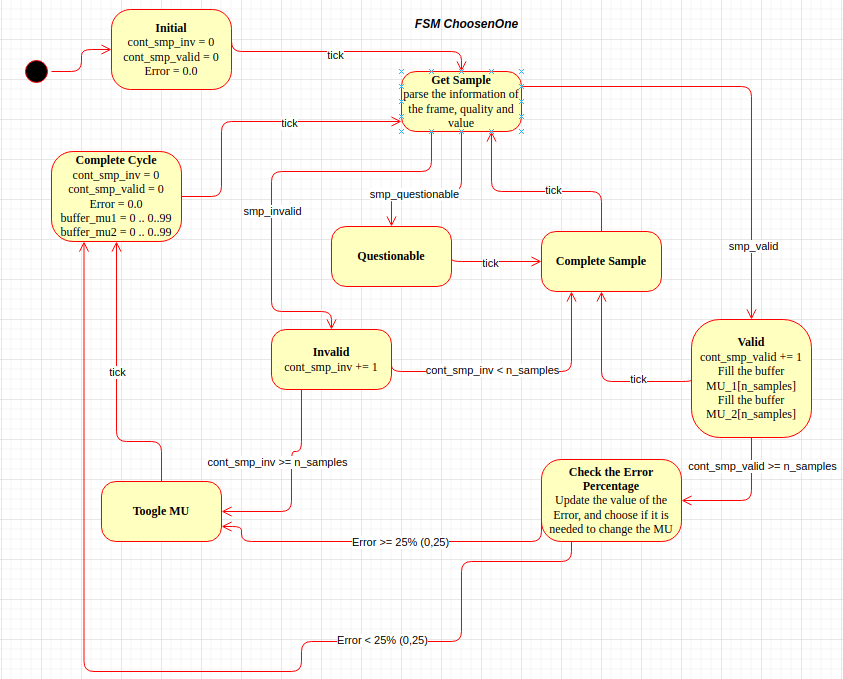
\includegraphics[width=0.95\textwidth, keepaspectratio]{ch4/assets/state_machine.png} % Reduce to 90% of the text width
	\caption{State Machine of Decision Make.}
	\label{fig:state_machine}
\end{figure}
%\FloatBarrier

The state machine is implemented in Rust and operates using two mechanisms for state transitions: events and ticks. Events are specific actions that trigger progress within the state machine, while ticks represent units of time. When a specified time elapses and the state requires only a tick to proceed, the machine advances, similar to how it transitions in response to events.
\begin{itemize}
	\item Initial State: This state runs only once when the algorithm is first executed. After this, the state can only be re-entered by a reset. After a tick, the state machine transitions to the 'Get Sample' state.
	\item Get Sample: In this state, the sample data is received, and information about the packet is processed. Based on the packet’s validity, the state machine decides to transition to one of three states: Valid, Invalid, or Questionable. The packet's status (valid, questionable, or invalid) determines the next state.
	\item Questionable: In the 'Questionable' state, no further action is taken other than validating the received packet. After a tick, the machine moves to the 'Complete Sample' state.
	\item Invalid: In the 'Invalid' state, the machine checks whether the number of valid packets received is below a defined threshold (n\_samples). If so, it advances to the 'Complete Sample' state; otherwise, it transitions to the 'Toggle MU' state.
	\item Valid: In the 'Valid' state, the system checks if the number of valid packets is below the threshold (n\_samples). If so, it transitions to the 'Complete Sample' state; otherwise, it moves to 'Check Error Percentage'. Additionally, the sample is placed in the appropriate index of the buffer, corresponding to the three-phase and neutral current and voltage measurements (Phase A to N) for the two MUs (Merging Units).
	\item Complete Sample: This state is essentially a waiting period, where the machine waits for a tick before transitioning back to the 'Get Sample' state.
	\item Toggle MU: In the 'Toggle MU' state, the Merging Unit is toggled, and the machine waits for a tick before transitioning to the 'Complete Cycle' state.
	\item Check Error Percentage: In this state, the entire buffer is evaluated to calculate the error percentage. If the error is below 25\%, the machine remains in the same MU and moves to the 'Complete Cycle' state. If the error exceeds 25\%, it transitions to the 'Toggle MU' state.
	\item Complete Cycle: In the 'Complete Cycle' state, all variables are reset to begin a new cycle of the algorithm. After resetting, the machine waits for a tick to return to the 'Get Sample' state.
\end{itemize}

This state machine ensures efficient processing and evaluation of sampled values from the Merging Units, adapting dynamically based on packet validity and system performance thresholds.

\begin{lstlisting}[caption={State Machine struct.}]
// Define the state machine
struct FrameProcessor {
	state: State,
	cont_smp_inv: u32,
	cont_smp_valid_sv_id_1: u32,
	cont_smp_valid_sv_id_2: u32,
	error_percentage: f32,
	buffer_mu1: [[i32; N_SAMPLES as usize]; 8], // buffer MU 1 current A,B,C and N - voltage A,B,C and N
	buffer_mu2: [[i32; N_SAMPLES as usize]; 8], // buffer MU 2 current A,B,C and N - voltage A,B,C and N
	toggle_mu: bool,
}
impl FrameProcessor {
	fn new() -> Self {
		Self {
			state: State::Initial,
			cont_smp_inv: 0, // Initialize cont_invalid
			cont_smp_valid_sv_id_1: 0,
			cont_smp_valid_sv_id_2: 0,
			error_percentage: 0.0,
			buffer_mu1: [[0 ; N_SAMPLES as usize]; 8],
			buffer_mu2: [[0 ; N_SAMPLES as usize]; 8],
			toggle_mu: false,
			
		}
	}
\end{lstlisting}

The diagram in Figure~\ref{fig:test_setup} illustrates the deployment of the software components on the hardware platforms.
The Merging Units and Protection Relay are simulated on the Jetson Nano node, while the Algorithm runs on the PC.
An Ethernet link connects the Merging Units to the Algorithm, and another Ethernet link connects the Algorithm to the Protection Relay.

The workflow is as follows:
\begin{enumerate}
	\item The MUs send sampled values (SV) to the Algorithm.
	\item The Algorithm analyses the received data and adaptively selects the best source.
	\item The Algorithm forwards the SV to the Protection Relay.
\end{enumerate}


\begin{figure}[tbh!]
	\centering
	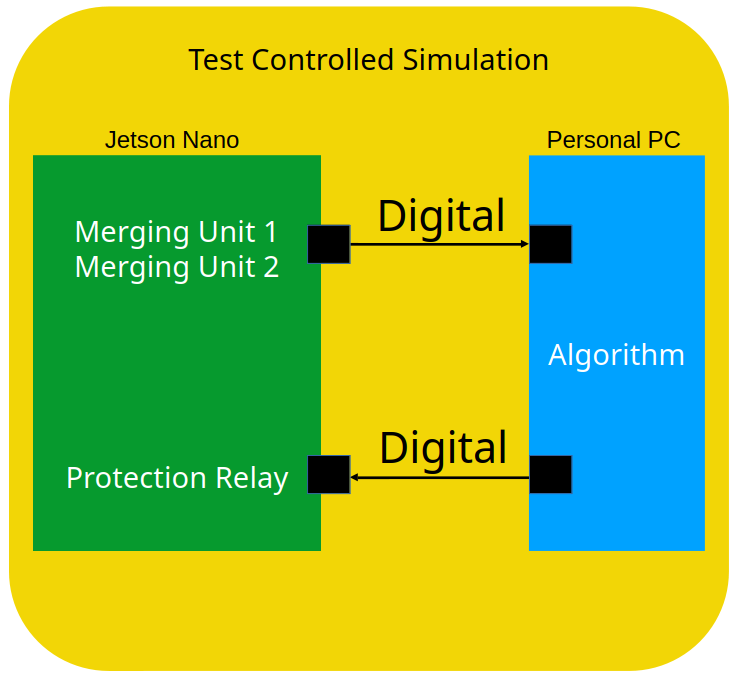
\includegraphics[width=0.70\textwidth, keepaspectratio]{ch4/assets/test_setup.png}
	\caption{How is connected the two simulators of SV's to exchange the information.}
	\label{fig:test_setup}
\end{figure}
%\FloatBarrier

All information regarding the development is available on GitHub, along with additional resources in the following location:

\hspace{1cm} \url{https://github.com/everton-oriente/IEC61850_9_2_SV}

% COMENTADO POR AMB
%These platforms collectively provide comprehensive access to the project's documentation, source code, and related materials.


\begin{comment}


\subsection{Results}

Leading the development and implementation of a communication protocol like IEC~61850-9-2 presented a completely different challenge. It required me to ensure that any other equipment connected to the network could understand exactly what was being sent. This involved understanding how operating systems handle network packets, the various headers that are added to ensure the information is properly routed and delivered to the correct destination, and how to assemble SV packets. The packets had to be sent in a way that the receiving application could correctly reassemble and interpret the data after it had been converted into bytes. This process required not only receiving and converting the bytes back into usable information within the IEC~61850-9-2 protocol but also ensuring that the destination equipment could understand the payload. Furthermore, it was critical to verify that the packet was intact and suitable for content analysis, while also maintaining synchronization between the two applications. This was particularly important given that the information needs to be transmitted every 250 microseconds, making network latency a critical factor.

The results obtained after all phases of development were satisfactory, considering the existing conditions. We used the Network Time Protocol (NTP) as the master clock, which provides a precision of 1 millisecond. However, achieving 100\% accuracy in timing was challenging because the protocol itself has a precision that exceeds the 250-microsecond interval at which we were transmitting the SV packets. Despite this limitation, the tests yielded values that were close to what was expected, demonstrating the feasibility of the models used. The ability to achieve such precision, even within these constraints, underscored the robustness and potential of the developed solution.

This experience not only deepened my technical understanding but also highlighted the complexities involved in real-time data transmission. It provided valuable insights into the challenges of ensuring data integrity, synchronization, and performance in real-time critical systems, where even the slightest delay or error can have significant consequences.

\end{comment}

\begin{comment}
\section{Roadmap}

The project plan has been meticulously developed following the waterfall approach. This structured methodology ensures that each phase of the project is completed before the next begins, providing a clear and organized progression. Table 4.1 outlines the distinct tasks required to achieve the research goals and objectives, along with their estimated duration, ensuring a systematic approach and timely completion of all critical activities.
I have used some tools as support like Project Libre.


\begin{table}[h]
	\centering
	\scriptsize
	\resizebox{\textwidth}{!}{
		\begin{tabular}{@{}lcccccccccc@{}}
			\toprule
			\textbf{Activities} & \textbf{Jan} & \textbf{Feb} & \textbf{Mar} & \textbf{Apr} & \textbf{May} & \textbf{Jun} & \textbf{Jul} & \textbf{Aug} & \textbf{Sep} & \textbf{Oct} \\ \midrule
			Research of articles                   & x & x &   &   &   &   &   &   &   &   \\
			Literature Review                      & x & x &   &   &   &   &   &   &   &   \\
			Development of Pré-Thesis              & x & x &   &   &   &   &   &   &   &   \\
			New Research of Articles               &   &   & x &   &   &   &   &   &   &   \\
			Decision Regarding development         &   &   & x &   &   &   &   &   &   &   \\
			Structure the Algorithm                &   &   & x &   &   &   &   &   &   &   \\
			Development of the Decision-Making Algorithm &   &   &   & x & x &   &   &   &   &   \\
			Test of the Decision-Making Algorithm  &   &   &   &   &   & x & x &   &   &   \\
			Write Thesis                           &   &   &   &   &   &   &   & x & x &   \\
			Conclusion and Results                 &   &   &   &   &   &   &   &   & x &   \\ 
			Defense of Master Thesis               &   &   &   &   &   &   &   &   &   & x \\
			\bottomrule
		\end{tabular}
	}
	\caption{Roadmap of activities}
	\label{table:roadmap}
\end{table}
\end{comment}


% Chapter 5

\chapter{Implementation} % Main chapter title

\label{chap:Chapter5} % For referencing the chapter elsewhere, use \ref{chap:Chapter5} 

%----------------------------------------------------------------------------------------

This chapter focuses on the development of the merging unit (publisher), the protection relay (subscriber), and algorithm essential to this project. It begins with Section 5.1, which explains the structure of SVs, laying the foundation for the algorithm's operation. Section 5.2 details the development of a publisher for IEC 61850-9-2-SV, covering data structuring, core function implementation, and testing through simulated signals. Section 5.3 addresses the development of a subscriber, highlighting the reuse of structures, data reception, error handling, and final implementation. The chapter also provides detailed insights into key portions of the code and the structures involved, particularly focusing on the state machine implemented to select the best sample of the analog signal. Finally, Section 5.4 discusses the overall development of the algorithm, integrating the components into a cohesive system and identifying the essential steps needed to advance the project. Initially, the path forward wasn't always clear, but as development progressed, the necessary methods and solutions were uncovered to ensure the successful completion of the project.

\section{Structure of Sampled Values}

\label{sec:Structure_of_Sampled_Values}
The IEC~61850-9-2 Sampled Values protocol operates based on the Ethernet standard, meaning the packet structure must follow that of Ethernet packets. As such, we have the preamble, destination MAC address, source MAC address, Ethertype, data, and FCS. However, since it's a SV packet, there is an additional field that isn't always present in all Ethernet standard packets: the Priority Tagging VLAN ID. This field must be included in the SV packet.

These elements are divided into the header, payload, and checksum. The header includes the Destination MAC address, Source MAC address, Priority Tagging VLAN ID, and Ethertype. The payload contains the Sampled Value Protocol Data Unit (SVPDU), which itself consists of the APPID, length, Reserved 1, Reserved 2, and the APDU. The APDU is made up of the savPDU, noASDU, SeqASDU, and ASDU, and within the ASDU, we have fields such as svID, smpCnt, confRev, smpSynch, SeqData, and the data. Finally, we have the FCS (Frame Check Sequence), which in this case uses CRC (Cyclic Redundancy Check). This ensures the frame is validated and the information is accurate.

Figure~\ref{fig:sv_packet_fields} Below in the figure has how it is compound the sampled values packets.~\footnote{\url{https://www.mdpi.com/1996-1073/12/19/3731}}.

\begin{figure}[tbh!]
\centering
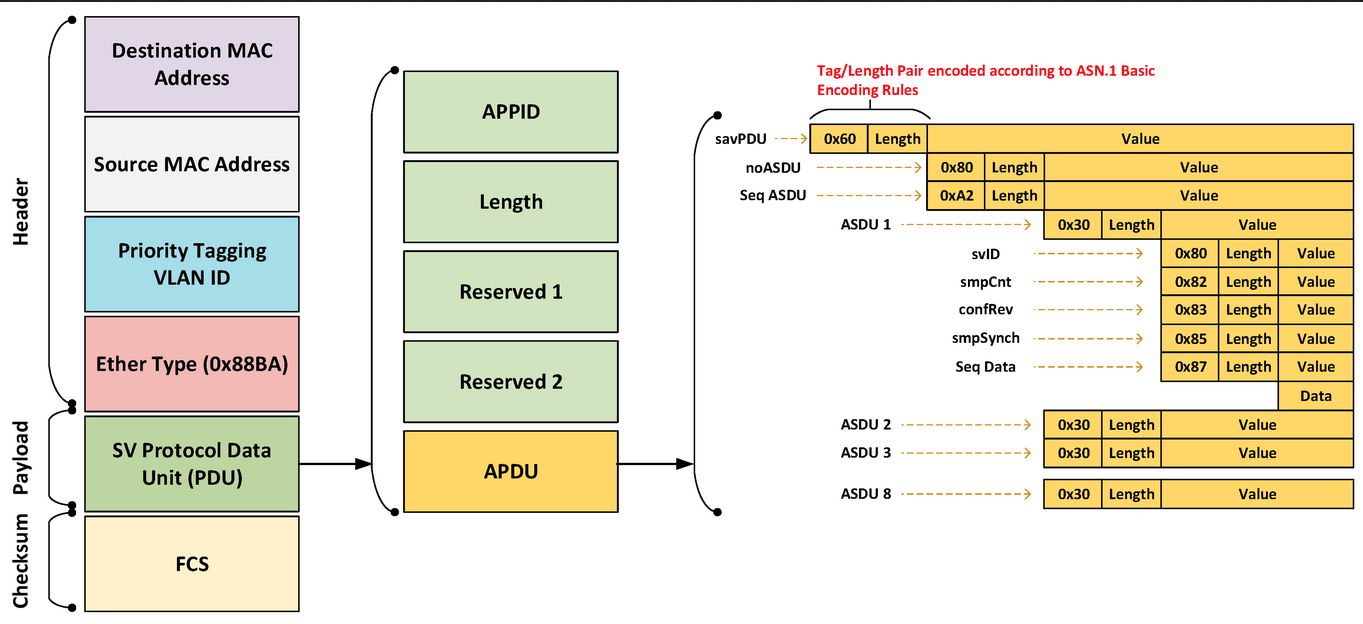
\includegraphics[width=0.95\textwidth, keepaspectratio]{ch5/assets/sv_packets_fields.png} % Reduce to 90% of the text width
\caption{Sampled Value packets fields. (Image credits: MDPI)}
\label{fig:sv_packet_fields}
\end{figure}
%\FloatBarrier

Following the recommendations of \cite{uca2024guideline}, the description is well documented in \textcite[Subsection 4.2]{IEC61850_KTH}, which explains this in detail.


Figure~\ref{fig:Sv_packet_full} Here has a representation of all the field until the values, and all the layers of the packet. \cite{uca2024guideline}

\begin{figure}[tbh!]
\centering
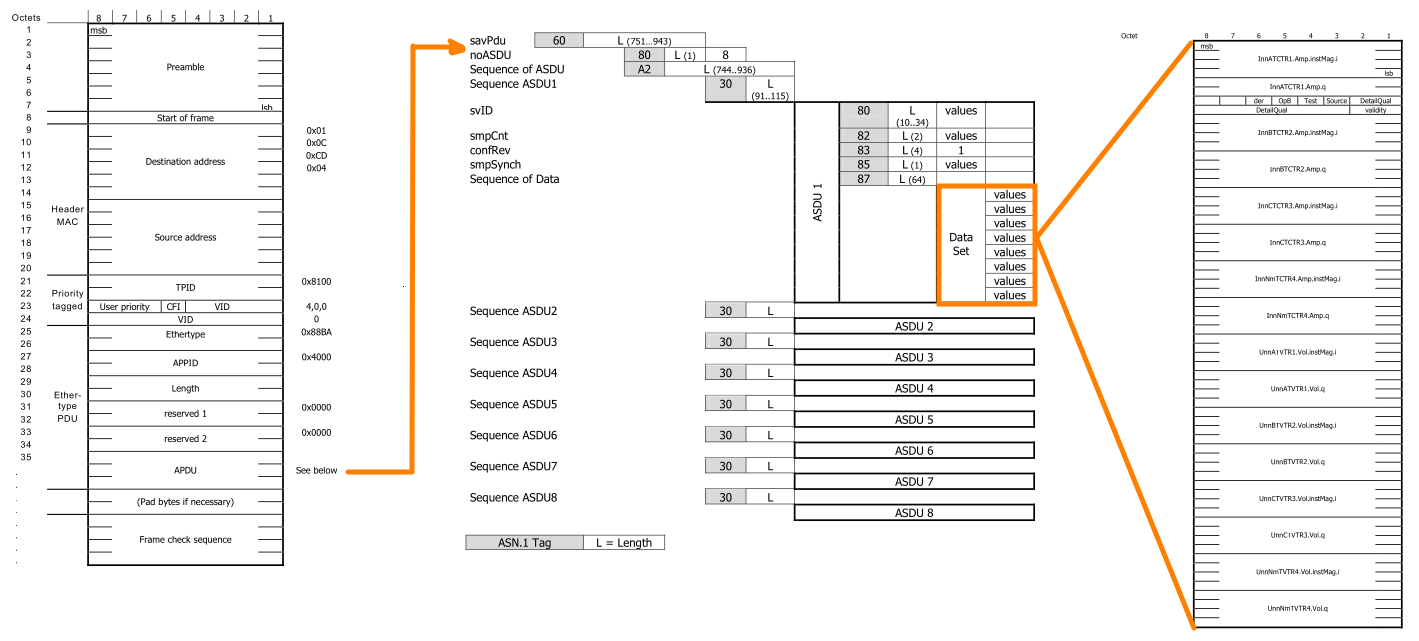
\includegraphics[width=0.95\textwidth, keepaspectratio]{ch5/assets/Sv_packet_full.png} % Reduce to 90% of the text width
\caption{Sampled Value packets fields. (Image credits: UCA International)}
\label{fig:Sv_packet_full}
\end{figure}
%\FloatBarrier

\section{Development of a Publisher of IEC~61850-9-2-SV}

The development of the publisher is a critical component in the implementation of the IEC~61850-9-2 Sampled Values communication standard. This section outlines the structured approach taken to build the publisher, focusing on the creation of key data structures (structs) and the implementation of essential functions that enable the generation and transmission of SV packets.

\subsection{Structuring the Data: Defining Rust Structs}

The process begins with defining the necessary structs. Rust, known for its strong emphasis on safety and concurrency, offers a well-organized way to build and manage complex data structures. This allows for clear and readable code, where each step of the data flow is defined in a sequence that is easy to understand and maintain.

The primary structs used in this project are designed to mirror the components of an Ethernet frame, as required by the IEC~61850-9-2 standard. These structs are nested to represent the hierarchy of the data, from the Ethernet frame down to the individual data points in the SV payload.


\begin{lstlisting}[caption={Structs added}]
pub struct EthernetFrame
{
pub destination:    [u8; 6],
pub source:         [u8; 6],
pub tpid:           u16,
pub tci:            u16,
pub ethertype:      u16,
pub payload:        SvPDU,
pub fcs:            [u8; 4],
}

pub struct SvPDU
{
pub appid:          [u8; 2],
pub length:         [u8; 2],
pub reserved1:      [u8; 2],
pub reserved2:      [u8; 2],
pub apdu: SmvData,
}

pub struct SmvData
{
pub sav_pdu_asn:    [u8; 2],
pub no_asdu_asn:    [u8; 2],
pub no_asdu:        u8,
pub seq_asdu_asn:   [u8; 2],
pub asdu_asn:       [u8; 2],
pub sv_id_asn:      [u8; 2],
pub sv_id:          [u32; 1],
pub smp_cnt_asn:    [u8; 2],
pub smp_cnt:        [u16; 1],
pub conf_rev_asn:   [u8; 2],
pub conf_rev:       [u32; 1],
pub smp_synch_asn:  [u8; 2],
pub smp_synch:      u8,
pub seq_data:       [u8; 2],
pub logical_node: LogicalNode,
}

pub struct LogicalNode
{
pub i_a:    [i32; 1],
pub q_ia:   [u32; 1],
pub i_b:    [i32; 1],
pub q_ib:   [u32; 1],
pub i_c:    [i32; 1],
pub q_ic:   [u32; 1],
pub i_n:    [i32; 1],
pub q_in:   [u32; 1],
pub v_a:    [i32; 1],
pub q_va:   [u32; 1],
pub v_b:    [i32; 1],
pub q_vb:   [u32; 1],
pub v_c:    [i32; 1],
pub q_vc:   [u32; 1],
pub v_n:    [i32; 1],
pub q_vn:   [u32; 1],
}
\end{lstlisting}

These structs allow for a comprehensive representation of the Ethernet frame and the SV data contained within, ensuring that each element of the SV packet is accurately captured and can be easily manipulated during transmission.

\subsection{Implementing the Core Functions}

Once the data structures are in place, the next step is to implement the functions that will operate on these structs. Rust uses the 'impl' keyword to define methods for structs, allowing for the creation of constructors, data manipulation functions, and other essential operations.

For example, the implementation of a constructor for the 'EthernetFrame' struct might look like this:

\begin{lstlisting}[caption={How to implement an impl for the struct}]
/ Implementation of functions regarding EthernetFrame struct
impl EthernetFrame {
pub fn new(destination: [u8; 6], source: [u8; 6], tpid: u16, tci: u16, ethertype: u16, payload: SvPDU, fcs: [u8; 4]) -> Self {
Self {
	destination,
	source,
	tpid,
	tci,
	ethertype,
	payload,
	fcs,
}
}
\end{lstlisting}

This function allows for the creation of a new EthernetFrame instance, ensuring that all necessary fields are initialized correctly.

\subsection{Simulating an Electrical Grid Signal}

A key functionality of the publisher is to simulate the sinusoidal signal of an electrical grid. This simulation is essential for generating realistic SV packets that can be used to test and validate the SV communication system.

To achieve this, the current time is used as an input to calculate the voltage and current values, with predefined amplitudes representing the electrical parameters. This simulation is implemented in the following function:

\begin{lstlisting}[caption={How to calculate the value of the SV's }]
pub fn cal_current_phase_b ()-> [i32;1]
{
let now = Local::now();
let t: f32 = now.timestamp_subsec_nanos() as f32 / 1_000_000_000.0;
let phase_degrees: f32 = 120.0; // Example phase in degrees
let phase_radians: f32 = phase_degrees * PI / 180.0; // Convert phase to radians
let omega: f32 = 2.0 * PI * FREQUENCY;
let amplitude: f32 = AMPLITUDE_CURRENT * ((omega * t + phase_radians).sin());
[amplitude as i32;1]
}
\end{lstlisting}

This function calculates the current value for phase B at a given moment, using the system's local time to simulate the progression of the sinusoidal wave. The result is an array containing the current value, which can then be included in the SV packet.

\subsection{Introducing Invalid Samples for Testing}

To fully test the algorithm's ability to handle real-world scenarios, it was necessary to introduce invalid samples. This was accomplished by altering the quality of certain samples within the SV packets, making them invalid. The publisher was enhanced with a feature that allows these quality changes, enabling the testing of how well the algorithm can identify and respond to invalid data.

\begin{lstlisting}[caption={How to calculate the value of the SV's }]
if increment > 50 \&\& increment < 100
{
// Implement Bad Quality to the samples
// The value of 0 is good quality
// The value of 1 and 2 is invalid
//The value of 3 it is questionable
sv_packet.payload.apdu.logical_node.q_ia[0] = sv_packet.payload.apdu.logical_node.q_ia[0].wrapping_add(1);	
}
\end{lstlisting}

This method directly modifies the 'sv\_packet.payload.apdu.logical\_node.q\_ia' field, effectively marking the sample as invalid. This invalid data can then be used to test the robustness of the SV communication and processing algorithm.

\subsection{Finalizing the Publisher}

With the basic structure, implementation, and testing features in place, the development of the publisher was completed. The final publisher is capable of generating and transmitting SV packets, simulating electrical grid signals, and introducing invalid data for testing purposes. These features are critical to the overall success of the thesis, as they enable comprehensive testing and validation of the IEC~61850-9-2 SV standard.

\section{Development of a Subscriber of IEC~61850-9-2-SV}

The development process for the subscriber followed a similar structured approach as that of the publisher. Having already established the necessary structs during the publisher's development, the focus for the subscriber shifted towards receiving and processing the data transmitted by the publisher over the network.

In this context, the subscriber was designed to handle incoming Sampled Values (SV) packets, log the received data, and print the relevant information to the log. This approach not only facilitated real-time monitoring of the transmitted SV data but also provided a foundation for verifying the integrity and accuracy of the data exchange between the publisher and subscriber.

\subsection{Structs Reused in the Subscriber}

Given that the subscriber's primary role is to interpret the data sent by the publisher, the same set of structs, including 'EthernetFrame', 'SvPDU', 'SmvData', and 'LogicalNode', were reused. These structs allowed the subscriber to decode the incoming Ethernet frames and extract the necessary information from the SV packets.

\begin{lstlisting}[caption={EthernetFrame struct. }]
	pub struct EthernetFrame {
		pub destination: [u8; 6],
		pub source: [u8; 6],
		pub tpid: u16,
		pub tci: u16,
		pub ethertype: u16,
		pub payload: SvPDU,
		pub fcs: [u8; 4],
}

// Other structs reused as shown in the publisher's code...
\end{lstlisting}

\subsection{Implementation of Data Reception and Logging}

The implementation phase involved creating functions to capture the network packets, parse them into the appropriate struct fields, and log the data for analysis. The impl blocks provided a seamless way to define these methods, ensuring that the subscriber could efficiently process the data.

\subsection{Error Handling and Invalid Data Processing}

An essential part of the subscriber’s functionality involved handling errors and invalid data. Similar to the publisher, where invalid samples were introduced to test the algorithm, the subscriber needed to identify and appropriately respond to these invalid samples. This was achieved by checking the quality of the received data and ensuring that any invalid samples were flagged and processed correctly.

\subsection{Finalizing the Subscriber}

By incorporating robust data reception, validation, and logging mechanisms, the subscriber was completed with the essential features required to support the overall thesis objectives. The subscriber was now fully equipped to interact with the publisher, process the received SV packets, and handle any errors or invalid data that might arise during transmission. This setup provided a solid foundation for testing and verifying the performance of the implemented communication protocol.

\section{Development of the Algorithm}

The development of the algorithm hinges on a deep understanding of both the publisher and subscriber functions. The aim is to create an algorithm capable of selecting the optimal samples from two independent devices that measure the same electrical quantity. This involves transmitting these measurements via a protocol, decompressing the data, extracting the necessary values, evaluating them, and ultimately selecting the best sample. All of this must be accomplished within a timeframe that ensures the Sampled Values (SVs) reach the protection devices without delay—each SV being transmitted every 250 microseconds.

The algorithm is triggered upon the reception of an SV from one of the merging units. Once received, the SV is processed and evaluated to determine whether it is valid, invalid, or questionable. If the sample is valid, its values are extracted for comparison with those from the other merging unit. In the case of an invalid or questionable sample, it is excluded from the value acquisition process. However, the algorithm keeps track of the number of invalid samples, which is one of the criteria used to decide whether to switch the SVs being sent to the protection relays.

For valid samples, a comparison is made on a sample-by-sample basis to ensure the best result. If the error does not exceed 25\%, the current SV is maintained; however, if the error surpasses 25\%, the SV being sent to the protection relays is switched. A state machine was implemented to make the decision on which SV to send to the protection devices. Although the system receives values from two merging units, only one of the two received SVs is transmitted.

\subsection{Algorithm Logic and Structure}

The core of the algorithm revolves around a decision-making structure that ensures reliable selection of SVs. The state machine is implemented to manage the comparison process and handle the switching of samples. Each incoming SV is processed in real time, where the following steps are taken:

\begin{itemize}
	\item Data Decompression: Upon reception of the SVs from the publisher, the algorithm first decompresses the data to retrieve the individual fields necessary for processing. These fields include the sample count (smpCnt), configuration revision (confRev), and the actual sampled values.
	\item Data Validation: Each Sampled Value undergoes an integrity check using a checksum before processing. If the sample is flagged as invalid or questionable in terms of quality, it is excluded from the comparison. This ensures that only trustworthy SVs are considered for further analysis, enhancing the reliability of the results.
	\item Comparison Between SVs: For valid SVs, the algorithm compares the sampled values from both merging units. If the absolute difference between the two SVs is within an acceptable threshold (25\%), the system continues using the current SV. If the difference exceeds this threshold, the algorithm triggers the switching mechanism.	
	\item Decision Process Using State Machine: The algorithm utilizes a state machine to manage the decision-making process for switching between Sampled Values. This system ensures that switching occurs only when the error between the two SVs exceeds a predefined threshold and a series of checks confirm that the alternative SV is more suitable for transmission. Additionally, the state machine monitors the data stream for invalid samples and initiates a switch if a persistent stream of invalid samples is detected, ensuring that the most accurate data is consistently transmitted.
\end{itemize}

\subsection{Handling Invalid and Questionable Samples}
Invalid or questionable SVs are handled by implementing a robust error-checking mechanism. The algorithm is designed to track the occurrence of invalid samples and make decisions accordingly. If a sample is deemed invalid, it is discarded from further evaluation, but the algorithm logs this occurrence to maintain an awareness of the merging unit's performance.

If invalid samples persist over a defined threshold, the state machine initiates a switch to the other merging unit. This mechanism ensures that the system continuously provides reliable SVs to the protection relays, even in cases where one merging unit is producing questionable data.

\subsection{Decision-Making Through Error Tracking and Switching}
The state machine tracks various error conditions, such as large deviations between SVs and a high number of invalid samples. The switching logic takes into account both real-time error tracking and historical data from previous SVs to decide whether to maintain the current sample or switch to the alternate SV.

The algorithm operates within a deterministic timeframe, where decisions must be made in under 250 microseconds to maintain real-time performance. This ensures that protection relays receive the most accurate and reliable data without introducing delays in decision-making.
% Chapter 6

\chapter{Tests and Evaluation} % Main chapter title

\label{chap:Chapter6} % For referencing the chapter elsewhere, use \ref{chap:Chapter6} 

%----------------------------------------------------------------------------------------

This chapter outlines the testing and evaluation processes crucial to achieving the project’s objectives. It begins with Section 6.1, which focuses on the tests conducted on the merging unit ()publisher of IEC 61850-9-2-SV, ensuring it performs accurately under various conditions. Section 6.2 details the testing of the subscriber, examining its ability to receive and process the data correctly. Finally, Section 6.3 evaluates the algorithm, particularly the state machine implemented to select the best sample of the analog signal. Throughout this chapter, rigorous testing approaches are emphasized, highlighting the steps taken to validate the algorithm's performance and secure the project's overall success. Initially, the testing path wasn’t entirely clear, but as it progressed, the necessary methods and solutions were identified to ensure the algorithm’s successful validation.

\section{Test of Publisher of IEC~61850-9-2-SV}

The testing phase for the publisher was critical to ensure its proper functionality, confirm that the data structures were correctly constructed, and verify that the checksum maintained packet integrity, all in strict compliance with the IEC~61850 standard.

Initial tests focused on validating that the publisher was generating Sampled Value (SV) packets accurately, with values consistent with the configured parameters. It was equally important to verify that the subscriber was correctly receiving and processing these transmitted packets. Wireshark software was extensively employed to capture and analyze the packets, ensuring that all content was transmitted as expected. Throughout development, several issues emerged, but each was methodically resolved to ensure the publisher's reliable performance and seamless communication.

Figure~\ref{fig:simple_sv} Below is a Wireshark capture that illustrates the integrity of the acquired packets and their identification as SV packets.

\begin{figure}[tbh]
	\centering
	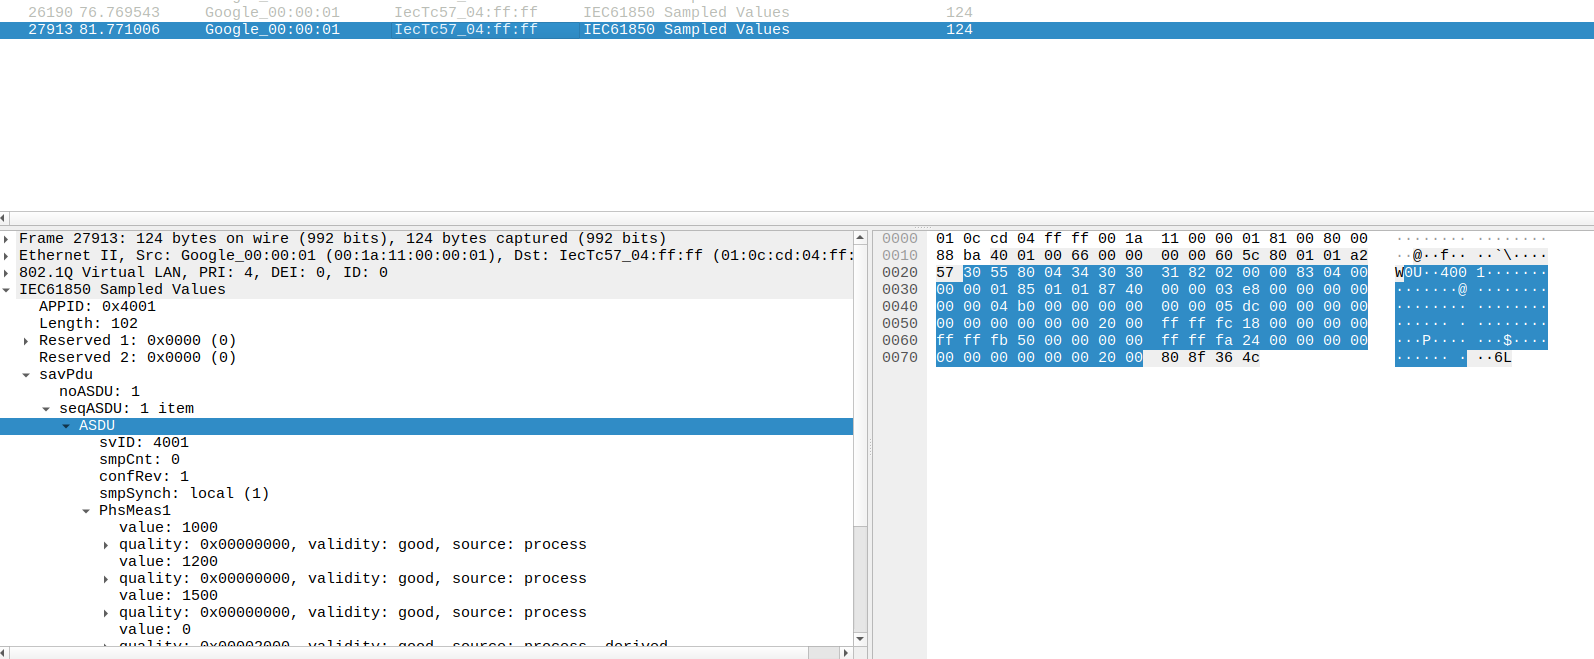
\includegraphics[width=1.00\textwidth, keepaspectratio]{ch6/assets/simple_sv.png} % Reduce to 90% of the text width
	\caption{Wireshark view of the SV packets.}
	\label{fig:simple_sv}
\end{figure}
\FloatBarrier

Figure~\ref{fig:sv_seq_1} The packets are sequentially numbered, ensuring proper identification. The following image demonstrates that the frames are correctly ordered, the field to check it is sample counter as smpcnt.

\begin{figure}[tbh]
	\centering
	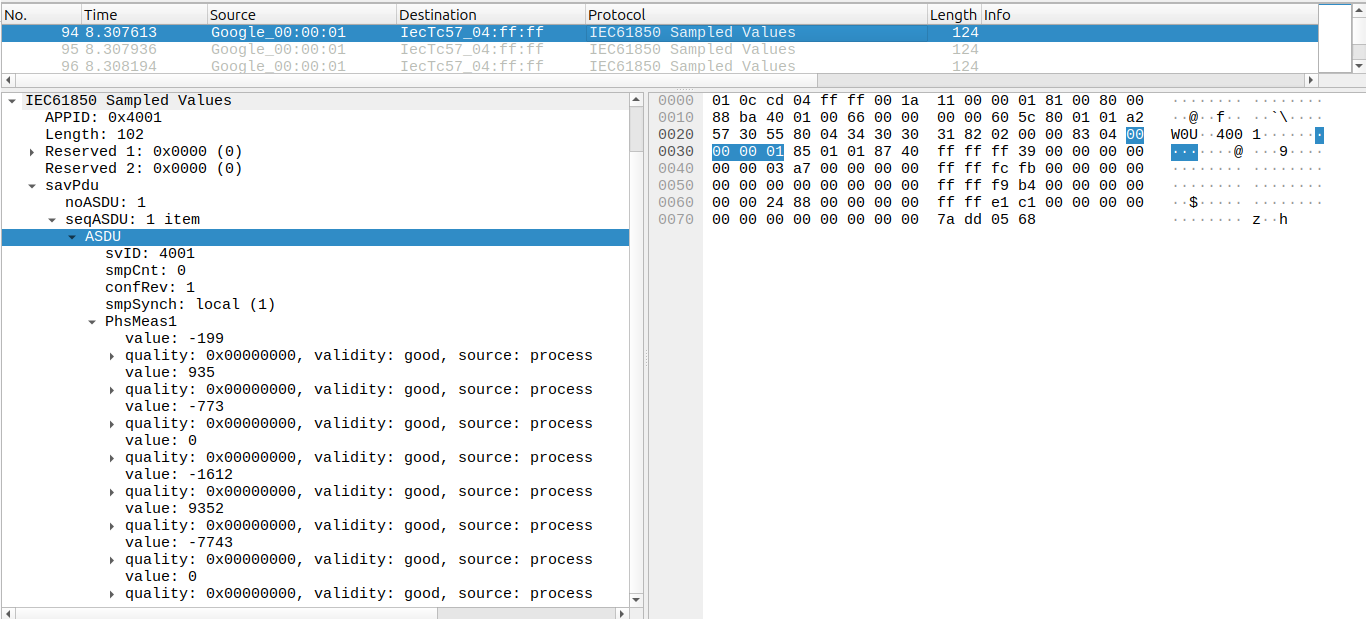
\includegraphics[width=1.00\textwidth, keepaspectratio]{ch6/assets/sv_seq_1.png} % Reduce to 90% of the text width
	\caption{SV packet with sample counter with value 0.}
	\label{fig:sv_seq_1}
\end{figure}
\FloatBarrier

\begin{figure}[tbh]
	\centering
	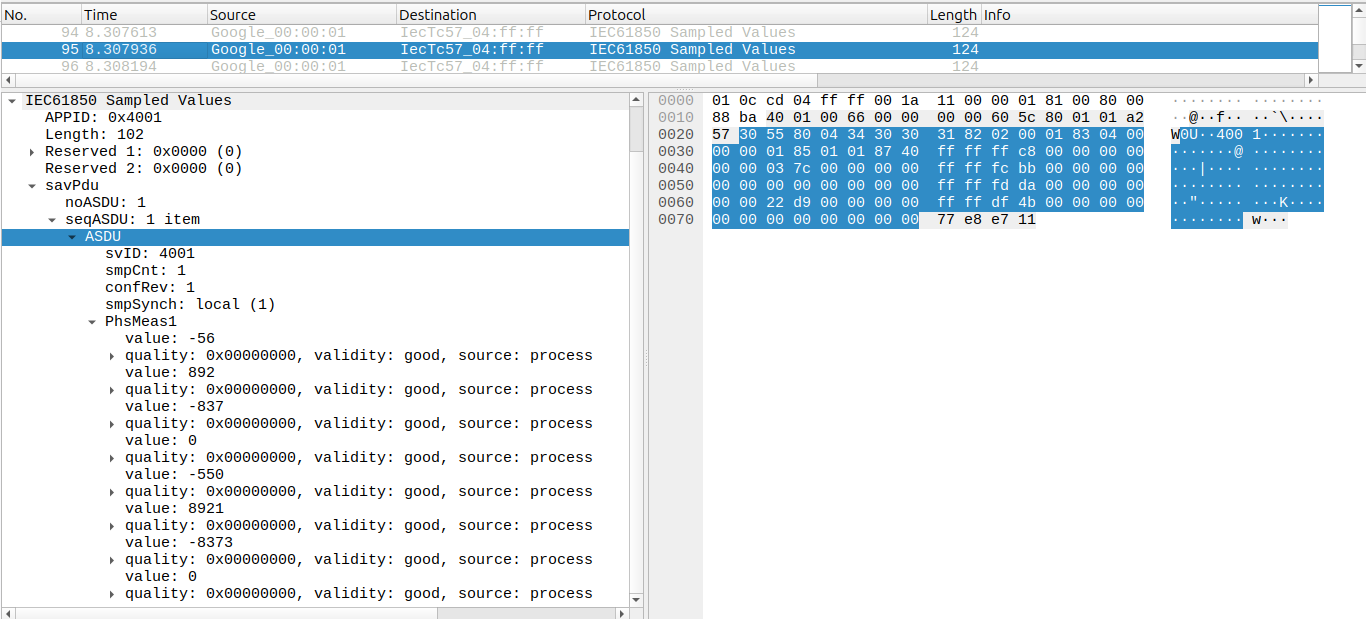
\includegraphics[width=1.00\textwidth, keepaspectratio]{ch6/assets/sv_seq_2.png} % Reduce to 90% of the text width
	\caption{SV packet with sample counter with value 1.}
	\label{fig:sv_seq_2}
\end{figure}
\FloatBarrier

\begin{figure}[tbh]
	\centering
	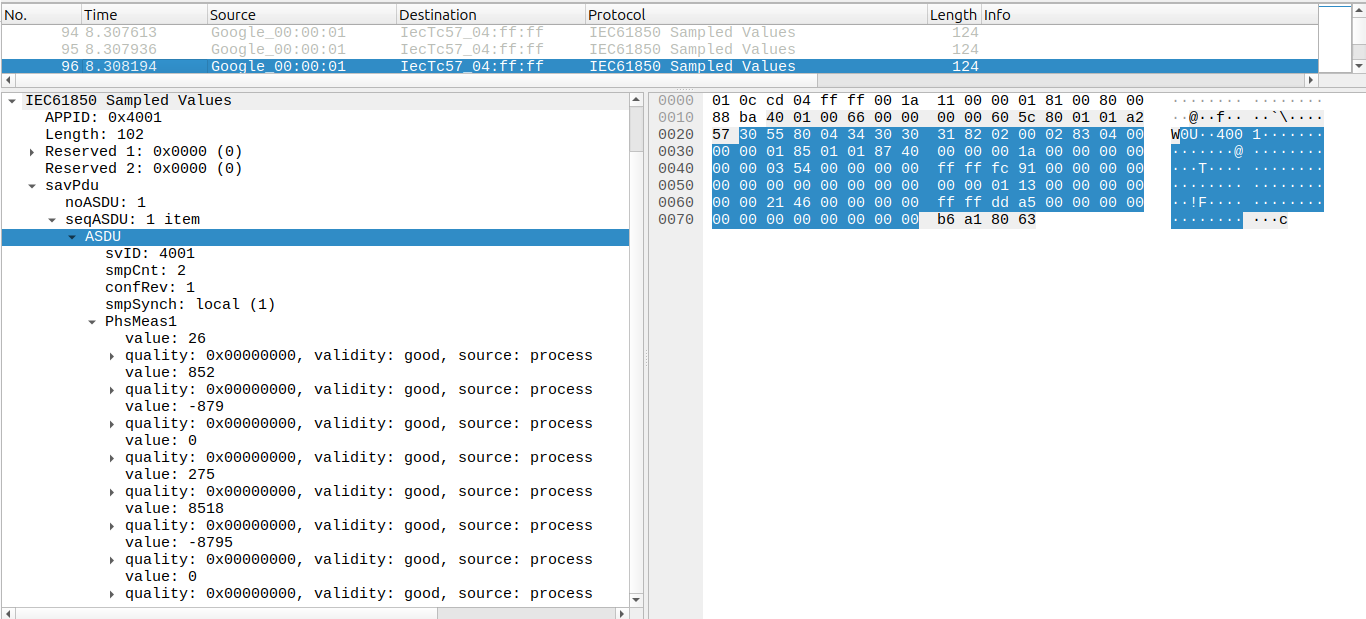
\includegraphics[width=1.00\textwidth, keepaspectratio]{ch6/assets/sv_seq_3.png} % Reduce to 90% of the text width
	\caption{SV packet with sample counter with value 2.}
	\label{fig:sv_seq_3}
\end{figure}
\FloatBarrier

Figure~\ref{fig:sv_seq_bad_1} Here, we showcase samples marked with bad quality, which were used to test the handling of invalid samples and trigger a switch to alternate samples received from another merging unit. The following images provide examples of the transmitted packets.

\begin{figure}[tbh]
	\centering
	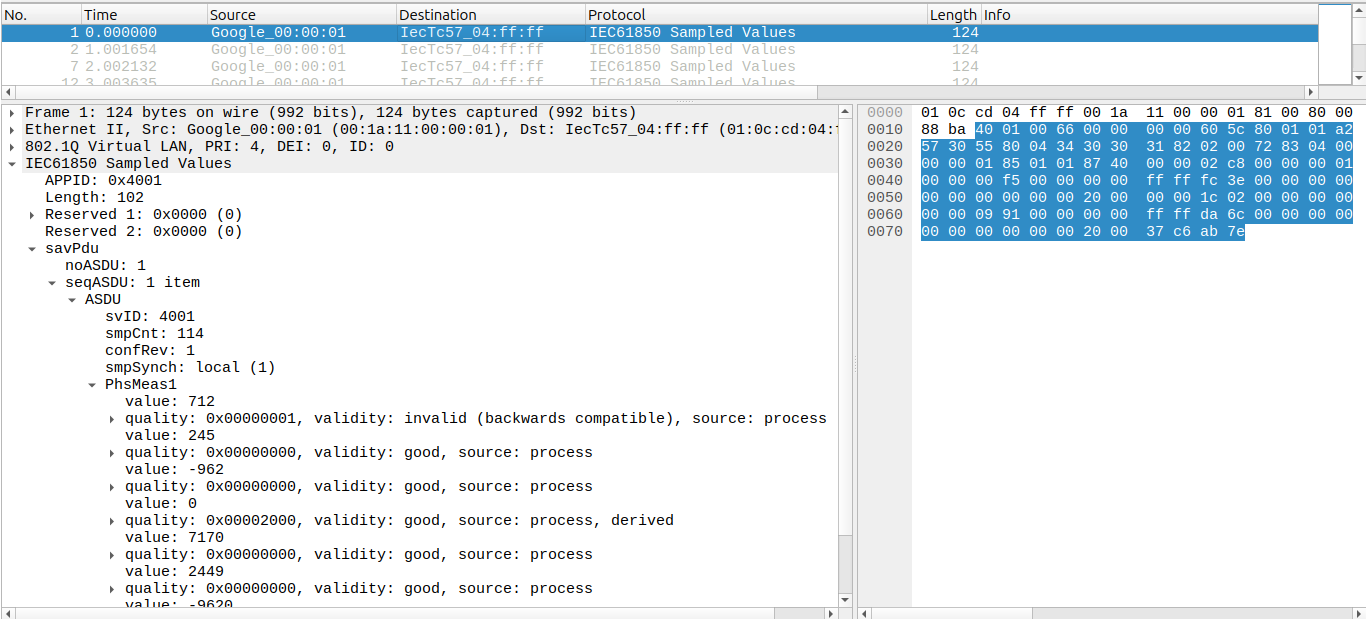
\includegraphics[width=1.00\textwidth, keepaspectratio]{ch6/assets/sv_seq_bad_1.png} % Reduce to 90% of the text width
	\caption{SV packet with bad quality sample counter with value 114.}
	\label{fig:sv_seq_bad_1}
\end{figure}
\FloatBarrier

\begin{figure}[tbh]
	\centering
	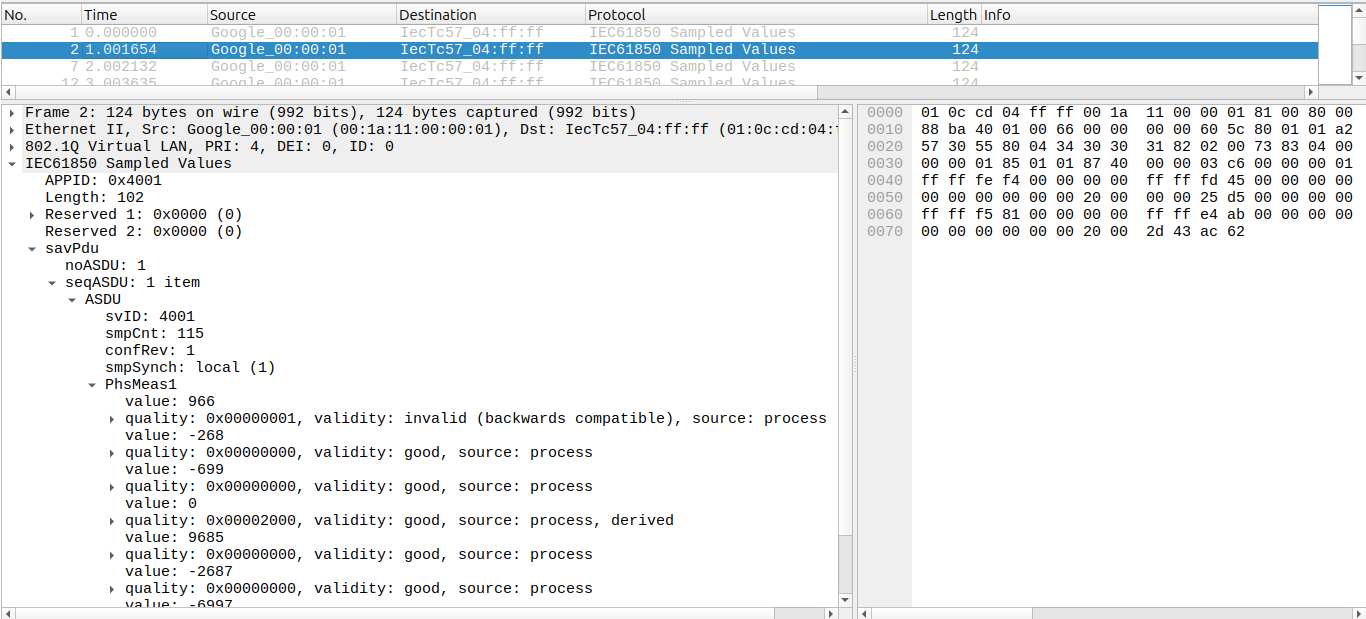
\includegraphics[width=1.00\textwidth, keepaspectratio]{ch6/assets/sv_seq_bad_2.png} % Reduce to 90% of the text width
	\caption{SV packet with bad quality sample counter with value 115.}
	\label{fig:sv_seq_bad_2}
\end{figure}
\FloatBarrier

These comprehensive tests confirm the publisher's correct functionality, ensuring reliable and accurate information exchange between different devices.  The three pictures above show a invalid in the field of quality of the samples, this means I have tested also the way through bad quality samples and ensure the algorithm change which Merging Unit is sending the SV packets, it is also possible to verify the sample counter to realize it is also in order the packets.

\section{Test of Subscriber of IEC~61850-9-2-SV}

The testing phase for the subscriber was essential to ensure it functioned correctly, accurately processed SV packets, and adhered to the IEC~61850 standard.

Initial tests focused on verifying that the subscriber could correctly receive and decode SV packets generated by the publisher. It was crucial to confirm that the subscriber subscribed to the data stream and processed the information as expected. Wireshark was extensively used to monitor and analyze the packet flow, and despite several challenges, each issue was promptly addressed to ensure reliable performance and seamless integration with the publisher.

Throughout testing, both Wireshark and application logs were used to carefully analyze every byte sent and received. This thorough inspection allowed for quick detection of inconsistencies and corrections. Initially, testing on the same machine concealed a problem that became evident only when packets were transmitted across a network: the VLAN information in SV packets was stripped by the operating system when sent to another device. This behavior is normal, as the VLAN data is only necessary for routing but doesn’t reach the application level. Understanding this behavior was crucial for addressing the issue and implementing a solution.

Once the core issues were resolved, testing confirmed the accurate exchange of data, ensuring each byte was correctly serialized and deserialized. This was vital since the state machine relies on precise data to make decisions. Any discrepancies would have caused failures or erratic behavior in the sample selection algorithm. The thorough testing guaranteed that the system operated as intended, free of errors.

Figure~\ref{fig:subscriber_side} Here, we have the wireshark sniffing the information at the subscriber side, and also one packet of the publisher and the subscriber side.

\begin{figure}[tbh]
	\centering
	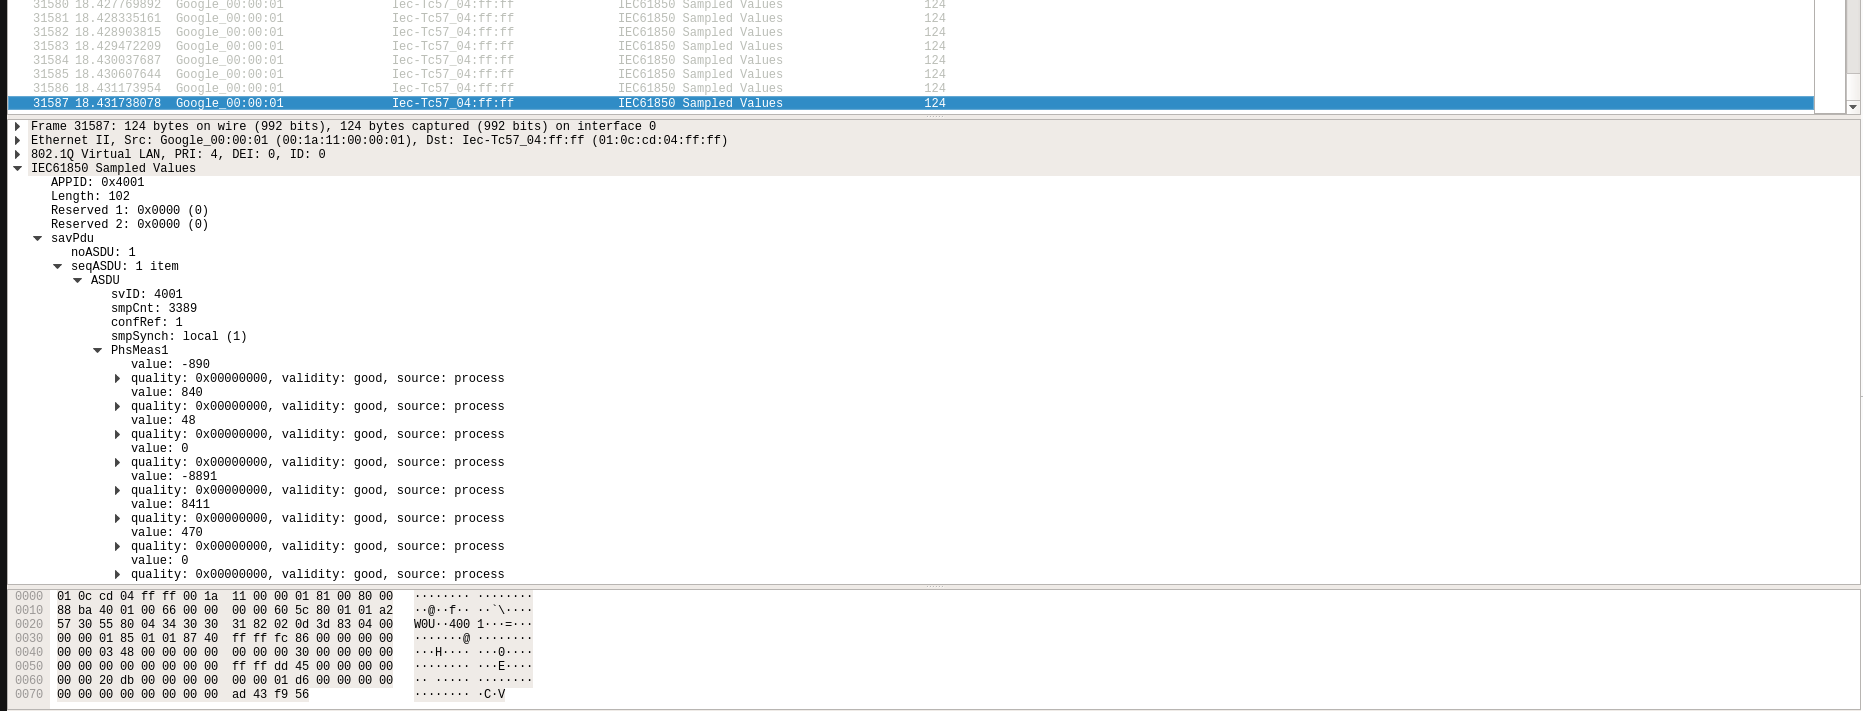
\includegraphics[width=1.00\textwidth, keepaspectratio]{ch6/assets/subscriber_side.png} % Reduce to 90% of the text width
	\caption{SV packet at subscriber side}
	\label{fig:subscriber_side}
\end{figure}
\FloatBarrier

\begin{figure}[tbh]
	\centering
	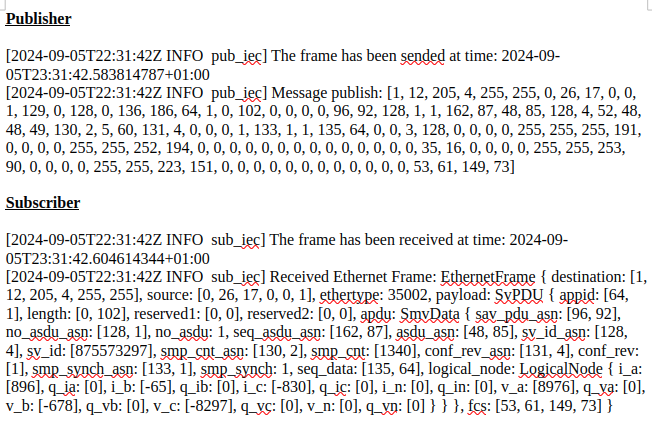
\includegraphics[width=0.85\textwidth, keepaspectratio]{ch6/assets/information_packet_sub_pub.png} % Reduce to 90% of the text width
	\caption{Information provided by Log of publisher and subscriber, the same packet in both equipment}
	\label{fig:information_packet_sub_pub}
\end{figure}
\FloatBarrier

Upon completing the tests, it was confirmed that the data sent by the publisher was correctly received and properly serialized by the subscriber, from the destination fields to the Frame Check Sequence (FCS).

However, an issue was identified during tests conducted on the same machine, where additional VLAN packets were processed by the subscriber. This occurred because, when running on the same system, the operating system does not discard VLAN data, as the packets don’t actually leave the machine. As a result, the data serialization became incorrect when the system was moved to a real-world test environment involving two separate devices communicating through network switches. In this scenario, the operating system on each device appropriately "consumes" the VLAN data, which is not needed beyond the network transmission phase.

After thorough investigation, it was determined that the VLAN packets should indeed be consumed by the operating system, as they are part of the lower layers in the OSI model. Recognizing this, we made the necessary adjustments to ensure proper data serialization when transferring packets across different devices in a networked environment, resolving the issue and ensuring reliable communication between publisher and subscriber.

\section{Test of the Algorithm}

This chapter outlines the testing of the code used by the algorithm and the evaluation process for achieving the project’s objectives. It provides a detailed description of the testing approach, with an emphasis on the steps taken to rigorously validate the algorithm's performance. Throughout the process, the necessary methods and solutions were identified to ensure the successful validation of the algorithm and the overall project.

With the development and testing of both the publisher and subscriber complete, the testing of the algorithm could begin, knowing that both components were functioning as expected. The initial tests focused on correctly serializing data and acquiring the necessary information for the state machine to progress and make decisions. The publisher was configured to generate valid, invalid, and questionable samples, ensuring that all states of the state machine could be tested. This comprehensive testing approach allowed for the verification and validation of transitions through all states, ensuring proper functionality.

The first trials followed the normal flow of the algorithm, as represented in Figure \ref{fig:state_machine}. The state machine is initialized and waits to receive a sample, which can be one of three types: Valid, Invalid, or Questionable. Initially, tests were conducted with Valid samples.

Once a valid sample is acquired, the state transitions to the Valid state. Within this state, both the tick transition and the condition cont\_smp\_valid >= n\_samples were tested. The state machine successfully transitioned to either the Complete Sample state or the Check the Error Percentage state. As the Complete Sample state processes all samples and returns to the Get Sample state, this scenario was tested multiple times and functioned correctly in all cases. This allowed us to move forward with testing the transitions related to the Check the Error Percentage state.

In the Check the Error Percentage state, the values in the buffer are evaluated. All values are summed, and a percentage is calculated. If this percentage exceeds 25\%, the state transitions to Toggle MU; otherwise, it proceeds to Complete Cycle. Multiple tests with values above and below this threshold were performed, and the state machine behaved correctly in all cases. The buffer values and percentages were analyzed to confirm the application's calculations, and the decision-making process was verified through implemented logs, ensuring that all transitions were accurate.

In the Toggle MU state, the SV packets sent to the protection devices are switched. If packets from Merging Unit 1 were being sent, the system switches to Merging Unit 2, and vice versa.

In the Complete Cycle state, all values are reset to their initial states, preparing the system for the next evaluation, where it determines whether or not to switch Merging Units.

The Initial state is responsible for initializing all necessary variables to zero, ensuring the process starts correctly.

When dealing with Invalid samples, the process begins in the Get Sample state, similar to Valid samples. After the analysis confirms the sample is invalid, the state transitions to Invalid. If the number of invalid samples exceeds n\_samples, the system moves to the Toggle MU state; otherwise, it transitions to Complete Sample.

Finally, for Questionable samples, the state machine simply waits for the tick and then transitions to Complete Sample. No additional handling is applied for questionable samples.

The following debug output captures the comprehensive testing of the state machine. This output provides a clear record of the testing process, illustrating how each message corresponds to various scenarios within the state machine. By tracing these messages, one can see the meticulous examination of every possible state and transition, ensuring that all functionalities were thoroughly validated. Additionally, the debug information offers insights into the algorithm's performance, demonstrating its ability to respond accurately to different conditions. This rigorous testing process was essential for confirming the reliability and effectiveness of both the state machine and the algorithm. Here are shown two examples of the state machine, when the samples are valid.

In the first scenario shown in Listing~\ref{lst:scenario1} the system acquires the data, checks if the quality is good, and then returns to collect another sample.

\begin{lstlisting}[caption={First scenario showing the steps through the state machine between the state Get Sample -> Valid, Valid -> Complete Sample -> Get Sample.}, label={lst:scenario1}]
[2024-07-14T18:22:50Z INFO  sub_with_fsm_iec] System ticked
[2024-07-14T18:22:50Z INFO  sub_with_fsm_iec] State: Initial
[2024-07-14T18:22:50Z INFO  sub_with_fsm_iec] System ticked
[2024-07-14T18:22:50Z INFO  sub_with_fsm_iec] State: Get Sample
[2024-07-14T18:22:50Z INFO  sub_with_fsm_iec] Verify Quality of the Sample
[2024-07-14T18:22:50Z INFO  sub_with_fsm_iec] Logical Node : 0
[2024-07-14T18:22:50Z INFO  sub_with_fsm_iec] Get Sample -> Valid
[2024-07-14T18:22:50Z INFO  sub_with_fsm_iec] System ticked
[2024-07-14T18:22:50Z INFO  sub_with_fsm_iec] State: Valid
[2024-07-14T18:22:50Z INFO  sub_with_fsm_iec] Value of Buffer MU 1 fase: 0 value: 558
[2024-07-14T18:22:50Z INFO  sub_with_fsm_iec] Value of Buffer MU 1 fase: 1 value: -997
[2024-07-14T18:22:50Z INFO  sub_with_fsm_iec] Value of Buffer MU 1 fase: 2 value: 443
[2024-07-14T18:22:50Z INFO  sub_with_fsm_iec] Value of Buffer MU 1 fase: 3 value: 0
[2024-07-14T18:22:50Z INFO  sub_with_fsm_iec] Value of Buffer MU 1 fase: 4 value: 5540
[2024-07-14T18:22:50Z INFO  sub_with_fsm_iec] Value of Buffer MU 1 fase: 5 value: -9980
[2024-07-14T18:22:50Z INFO  sub_with_fsm_iec] Value of Buffer MU 1 fase: 6 value: 4446
[2024-07-14T18:22:50Z INFO  sub_with_fsm_iec] Value of Buffer MU 1 fase: 7 value: 0
[2024-07-14T18:22:50Z INFO  sub_with_fsm_iec] The value of counter_sample_valid_of_sv_id_MU1: 1
[2024-07-14T18:22:50Z INFO  sub_with_fsm_iec] Valid -> CompleteSample
[2024-07-14T18:22:50Z INFO  sub_with_fsm_iec] System ticked
[2024-07-14T18:22:50Z INFO  sub_with_fsm_iec] State: CompleteSample
[2024-07-14T18:22:50Z INFO  sub_with_fsm_iec] CompleteSample -> GetSample
[2024-07-14T18:22:50Z INFO  sub_with_fsm_iec] Mu0 after evaluation
[2024-07-14T18:22:50Z INFO  sub_with_fsm_iec] Time of work of thread is: 287.475447ms
[2024-07-14T18:22:50Z INFO  sub_with_fsm_iec] Mu0 before evaluation
\end{lstlisting}

In the second scenario shown in Listing~\ref{lst:scenario2}, once the error percentage threshold is reached, the system decides whether to stay with the same MU or switch to a different one. In this case, the scenario demonstrates switching the MU.

\begin{lstlisting}[caption={Second scenario showing the steps through the state machine between the state Get Sample -> Valid, Valid -> Check the Error Percentage -> Toogle MU -> Complete Cycle -> Get Sample.}, label={lst:scenario2}]
[2024-07-14T18:22:59Z INFO  sub_with_fsm_iec] System ticked
[2024-07-14T18:22:59Z INFO  sub_with_fsm_iec] State: Get Sample
[2024-07-14T18:22:59Z INFO  sub_with_fsm_iec] Verify Quality of the Sample
[2024-07-14T18:22:59Z INFO  sub_with_fsm_iec] Logical Node : 0
[2024-07-14T18:22:59Z INFO  sub_with_fsm_iec] Get Sample -> Valid
[2024-07-14T18:22:59Z INFO  sub_with_fsm_iec] System ticked
[2024-07-14T18:22:59Z INFO  sub_with_fsm_iec] State: Valid
[2024-07-14T18:22:59Z INFO  sub_with_fsm_iec] Value of Buffer MU 2 fase: 0 value: 935
[2024-07-14T18:22:59Z INFO  sub_with_fsm_iec] Value of Buffer MU 2 fase: 1 value: -167
[2024-07-14T18:22:59Z INFO  sub_with_fsm_iec] Value of Buffer MU 2 fase: 2 value: -769
[2024-07-14T18:22:59Z INFO  sub_with_fsm_iec] Value of Buffer MU 2 fase: 3 value: 0
[2024-07-14T18:22:59Z INFO  sub_with_fsm_iec] Value of Buffer MU 2 fase: 4 value: 9376
[2024-07-14T18:22:59Z INFO  sub_with_fsm_iec] Value of Buffer MU 2 fase: 5 value: -1678
[2024-07-14T18:22:59Z INFO  sub_with_fsm_iec] Value of Buffer MU 2 fase: 6 value: -7697
[2024-07-14T18:22:59Z INFO  sub_with_fsm_iec] Value of Buffer MU 2 fase: 7 value: 0
[2024-07-14T18:22:59Z INFO  sub_with_fsm_iec] The value of counter_sample_valid_of_sv_id_MU2: 5
[2024-07-14T18:22:59Z INFO  sub_with_fsm_iec] Valid -> CheckErrorPercentage
[2024-07-14T18:22:59Z INFO  sub_with_fsm_iec] System ticked
[2024-07-14T18:22:59Z INFO  sub_with_fsm_iec] State: CheckErrorPercentage
[2024-07-14T18:22:59Z INFO  sub_with_fsm_iec] Value of the error: 1.2880255
[2024-07-14T18:22:59Z INFO  sub_with_fsm_iec] Actual State: ToogleMU
[2024-07-14T18:22:59Z INFO  sub_with_fsm_iec] System ticked
[2024-07-14T18:22:59Z INFO  sub_with_fsm_iec] State: ToogleMU
[2024-07-14T18:22:59Z INFO  sub_with_fsm_iec] Toogle_MU before is : false
[2024-07-14T18:22:59Z INFO  sub_with_fsm_iec] Toogle_MU after is : true
[2024-07-14T18:22:59Z INFO  sub_with_fsm_iec] ToogleMU -> CompleteCycle
[2024-07-14T18:22:59Z INFO  sub_with_fsm_iec] System ticked
[2024-07-14T18:22:59Z INFO  sub_with_fsm_iec] State: CompleteCycle
[2024-07-14T18:22:59Z INFO  sub_with_fsm_iec] CompleteCycle -> GetSample
\end{lstlisting}

% Chapter 7

\chapter{Conclusion} % Main chapter title

\label{chap:Chapter7} % For referencing the chapter elsewhere, use \ref{chap:Chapter7} 

%----------------------------------------------------------------------------------------

\section{Conclusions and Final Considerations}

This project originated from a critical need in the energy industry. As substations evolve into the digital age, merging units have been introduced to digitize the acquisition of current and voltage measurements. Today, redundancy in communication networks ensures that if one network fails, data samples and communications seamlessly continue over an alternate network, safeguarding the integrity of the substation's protection systems.

Similarly, the concept of redundancy was applied to Sampled Values (SVs). Two different devices acquire the same analog data and publish it digitally. In this setup, two merging units simultaneously measure the same current and voltage transformers and publish the data. This enables the protection system to select one of the two samples for its algorithms, discarding the other. Currently, no selection mechanism exists, and only the first merging unit’s sample is used. The second unit’s sample is only considered if the first fails.

In response to these market challenges, this thesis focused on developing an algorithm that selects the best sample from two merging units measuring the same physical quantities, such as current and voltage, rather than defaulting to one unit. By comparing and choosing the optimal signal, the system not only provides a reliable backup but also improves the accuracy and efficiency of protective relays. This approach enhances decision-making in electrical protection systems, ultimately improving overall reliability and performance.

The development of a publisher and subscriber became necessary due to the lack of existing libraries for the IEC61850 protocol. This project opens the door for the use of the RUST programming language in creating digital-era equipment like Merging Units and Protection Relays. During my research, I found libraries available in languages such as C/C++, C\#, Java, Python, and Go. However, since no library existed for RUST, it was essential to build these components from the ground up, resulting in a solid and well-structured foundation that adheres to the IEC61850 standard.

The features implemented cover the core functionality of a Merging Unit, including the reading of analog values, which are automatically generated based on time with a fixed amplitude. This allows for value emulation, with the possibility of integrating an ADC (Analog to Digital Converter) in the future for real analog acquisition. The system also includes the creation and transmission of SV packets, though it currently lacks a more accurate time synchronization protocol. Presently, the setup uses NTP for time acquisition, but PTP, which offers greater precision and complies with IEC61850-9-2, would be the ideal solution.

In terms of protection relays, basic functionality was established, including the reception of SV packets. However, further development is needed to create a fully functional protection relay. The starting point for such a device is acquiring the SVs, after which data processing, protection algorithms, and the necessary actions, like operating the circuit breaker, can be applied.

In summary, this project represents a major step toward developing a system that, with further refinement, could be transformed into a product ready for use in the energy industry. These two components play key roles in the operation, maintenance, and prevention of issues within substations. This project introduces a new way of developing products using a previously untapped language in this domain, offering substantial value to the broader community.

\section{Limitations}

This project has its limitations, as the typical environment for a Merging Unit involves fiber optic communications at rates of 1 Gbps or higher, along with switches capable of high transfer rates and extremely low latencies. These conditions are crucial because Merging Units need to deliver samples every 250 microseconds. As a result, the latency must be less than this value to ensure timely packet delivery. However, in this setup, the time between sending and receiving packets exceeds 250 microseconds. Although the publisher transmits information every 250 microseconds, the subscriber receives it after a longer delay due to the latency of the setup I was able to develop. While no packets are lost, the reading speed is slower than desired, with the subscriber receiving data beyond the 250-microsecond target.

Another limitation is the synchronization between the publisher and the subscriber. Currently, the devices are synchronized via Network Time Protocol (NTP), providing minimal synchronization. However, the error margin with NTP is about 1 millisecond. Since we are dealing with samples in the microsecond range, NTP does not offer the precision required for accurate synchronization. Achieving higher precision would require the implementation of Precision Time Protocol (PTP), which provides resolution in the nanosecond range.

Finally, there is a hardware platform limitation. The devices used were a Jetson Nano 4GB and a personal computer, both of which come with inherent performance constraints, especially concerning Ethernet network performance. In both cases, it was necessary to add a USB-to-Ethernet adapter to provide two Ethernet ports for communication between the publisher/algorithm and the algorithm/subscriber.

\section{Future Work}

\subsection{Add an ADC to acquire values of Voltage Transformer and Current Transformer}

The merging unit was tested using simulated values to demonstrate proof of concept, but in real-world applications, an ADC is required to accurately measure signals from Voltage Transformers (VT) and Current Transformers (CT). While simulations validate initial functionality, testing with real equipment is essential for a reliable assessment of performance.

In modern protection relay systems, ADCs often face the challenge of processing signals with varying power levels, such as one weak and one strong. Traditionally, ADC resolution has been evaluated using single-signal scenarios, focusing on quantization noise and signal-to-noise ratio (SNR). However, this approach does not adequately address the complexity of handling multiple signals with large dynamic ranges. As noted by Laporte et al. (~\cite{laporte2024adc}), previous evaluation methods either underestimate or overestimate the resolution required in dual-signal scenarios.

The authors propose a new method for calculating the necessary ADC resolution by accounting for the interaction between weak and strong signals, demonstrating that this interaction can enhance the dynamic range beyond what older models predicted. Despite improvements in ADC technology, current 12- or 14-bit ADCs remain insufficient for many modern protection relay applications, where dynamic ranges of up to 130 dB are required. The authors suggest that techniques such as companding may be necessary to overcome these limitations.

This analysis is particularly relevant to the system under development, where both weak and strong signals are processed, requiring a thorough understanding of ADC resolution to ensure reliable performance in substation automation systems.

\subsection{Add a PTP server regarding the IEC61850-9-3-PTP}

Substations have evolved over the years and transitioned into the digital era, synchronization protocols have become increasingly essential to ensure the proper alignment of IED (Intelligent Electronic Device) events. This synchronization allows for an accurate understanding of the event sequence in case of a fault, providing clarity on what occurred at the substation. When all devices are synchronized to a common time source, it becomes possible to interpret events chronologically. The introduction of the IEC 61850 protocol established several options for generating the master clock, including IRIG-B, DCF 77, 1PPS, Serial ASCII, NTP, and PTP.

Among these, only NTP and PTP can use the existing Ethernet network for synchronization, while the others require separate electrical wiring. This made NTP popular and widely adopted as a "standard" synchronization protocol because it leverages the same Ethernet network used by IEC 61850 and offers sufficient resolution with millisecond accuracy, which was adequate for most substation applications before the advent of Merging Units. NTP was sufficient for other substation events like GOOSE, MMS, and signaling.

However, the introduction of PTP (Precision Time Protocol) brought higher precision, which became necessary with the use of Sampled Values, Synchrophasor measurements, and Travelling Wave Fault Location. These applications demand precision at the level of 100 microseconds or better, down to 1 microsecond, with PTP providing nanosecond-level accuracy. Consequently, PTP became essential for synchronization only after these advanced applications were implemented, and it was incorporated into the IEC 61850 standard starting in 2015. Further improvements were made with PTPv3 in 2019, which is compatible with PTPv2.

Looking ahead, there is an opportunity to enhance this project by implementing PTP to align the publisher with the IEC 61850-9-3 protocol. This will ensure the required time resolution for the Sampled Values published by the merging unit developed in this thesis (~\cite{baumgartner2024iec}).
			
\subsection{Implement a more secure Sampled Value (SV) packet in modern substations}

SV packets are critical in IEC 61850 substation automation systems (SAS), used to transmit digitized current and voltage measurements between various devices, such as Merging Units (MUs), Protection IEDs, and Control IEDs. These packets enable real-time decision-making to protect and control the grid infrastructure. However, as modern substations adopt networked communication, SV packets are exposed to various cybersecurity risks. Vulnerabilities, such as replay attacks and masquerade attacks, pose significant threats to the integrity of these messages, potentially leading to malfunctions in protection relays and equipment failures(~\cite{hussain2024security}).

The need for secure SV messages in automated substations stems from the following requirements:
\begin{itemize}
	\item Confidentiality: Ensuring that the data in SV packets cannot be accessed or altered by unauthorized entities.
	\item Integrity: Guaranteeing that the SV packet content has not been tampered with during transmission.
	\item Authentication: Confirming that the SV message originated from a legitimate source. 
	\item Timeliness: Ensuring that security measures do not introduce delays that would impact the system's ability to respond to faults in real-time(~\cite{hussain2024security}).
\end{itemize}

So implement a more secure way the SV packets is possible thorugh this 4 principles, Message Authentication Code (MAC), Encryption of SV Payload, Timestapping for replay attack mitigation and extension fields for security mechanism following by order:
\begin{itemize}
	\item Message Authentication Codes (MAC): A Message Authentication Code (MAC) provides a way to ensure both the integrity and authentication of SV messages. A MAC is generated using a cryptographic algorithm based on the contents of the message and a shared secret key between the publisher (Merging Unit) and subscriber (Protection IED)(~\cite{hussain2024security}).
	\item Encryption of SV Payload: Encryption ensures confidentiality, preventing unauthorized entities from reading the SV message contents. Advanced Encryption Standard (AES-GCM) is recommended for securing SV messages, as it supports both encryption and authentication in one operation(~\cite{hussain2024security}).
	\item Timestamping for Replay Attack Mitigation: Replay attacks involve capturing legitimate SV packets and resending them to trick the system into accepting outdated data as current. To mitigate this, each SV message must carry a timestamp that reflects the time the message was created(~\cite{hussain2024security}).
	\item Extension Fields for Security Mechanisms: Modifications to the SV message frame are required to support these security mechanisms. The IEC 61850-9-2 message format allows for an Extension field, which can be used to carry MAC values, encrypted payloads, and timestamps(~\cite{hussain2024security}).
\end{itemize}

Implementing a secure SV messaging scheme in IEC 61850 substations is essential to protect against modern cyber threats like replay and masquerade attacks. The combination of MAC for integrity and authentication, AES-GCM for encryption, and timestamping for replay attack prevention ensures that SV packets are protected against tampering and unauthorized access. While these enhancements increase the packet size and computational overhead, tests show that they can be implemented without compromising the real-time performance of protection systems. With the right key management practices and adherence to the IEC 62351 standard, secure SV messaging can significantly enhance the resilience and safety of automated substations(~\cite{hussain2024security}).




%----------------------------------------------------------------------------------------
%	BIBLIOGRAPHY
%----------------------------------------------------------------------------------------

\printbibliography[heading=bibintoc]

%----------------------------------------------------------------------------------------
%	THESIS CONTENT - APPENDICES
%----------------------------------------------------------------------------------------

%\appendix % Cue to tell LaTeX that the following "chapters" are Appendices

% Include the appendices of the thesis as separate files from the Appendices folder
% Uncomment the lines as you write the Appendices

%% Appendix A

\chapter{Guidelines to adapt the template for the Thesis Research Plan} % Main appendix title

\label{AppendixA} % For referencing this appendix elsewhere, use \ref{AppendixA}

The dissertation template document can be adapted for the Thesis Research Plan report, using the following guidelines:
\begin{itemize}
\item Change “Dissertation submitted in partial fulfilment of the requirements for the Master’s degree in Critical Computing Systems Engineering” to “Thesis Research Plan of the Master’s degree in Critical Computing Systems Engineering”.
\item	Remove the reference to the Jury.
\item	Remove unnecessary sections such as dedication, acknowledgement, etc.
\item	The Introduction and state-of-the-art chapters can provide the initial contents of the dissertation, which can be later evolved and extended in the Thesis work.
\item	Introduce a chapter after state-of-the-art with preliminary information on the proposed approach(es) to solve the identified problem. 
\item	Provide a chapter on the research plan for the second semester, including the work methodology (with necessary reference to evaluation of the work) and the proposed timeline.
\end{itemize}

%\input{appendices/appendixB}
%\input{appendices/appendixC}

%----------------------------------------------------------------------------------------

\end{document}
